%# -*- coding: utf-8-unix -*-
% !TEX program = xelatex
%%==================================================
%% thesis.tex
%%==================================================

\documentclass[bachelor, openany, twoside]{ssputhesis}

% 逐个导入参考文献数据库
\addbibresource{bib/thesis.bib}

%# -*- coding: utf-8-unix -*-
% !TEX program = xelatex
% !TEX root = ../thesis.tex
% !TEX encoding = UTF-8 Unicode
%TC:ignore
\title{基于Latex的论文模版}
\author{某\quad{}某}
\advisor{某某老师}
% \coadvisor{某某教授}
\defenddate{2019年5月8日}
\coursename{某某课程}
\school{上海第二工业大学}
\institute{某某学部}
\studentnumber{12345678901}
\cnacademicdegree{工学硕士}
\major{某某专业}
\class{某某班级}
\entrancetime{某某级}
\keywords{SSPU;Latex;论文}

\englishtitle{iOS-Based Task Plan and Time Management System}
\englishauthor{\textsc{Mo Mo}}
\englishadvisor{Prof. \textsc{Mou Mou}}
% \englishcoadvisor{Prof. \textsc{Uom Uom}}
\englishschool{Shanghai Jiao Tong University}
\englishinstitute{\textsc{Depart of XXX, School of XXX} \\
  \textsc{Shanghai Jiao Tong University} \\
  \textsc{Shanghai, P.R.China}}
\englishinstitutemaster{Depart of XXX, \\ School of XXX}
\englishmajor{A Very Important Major}
\englishdate{Dec. 17th, 2014}
\enacademicdegree{Master of Engineering}
\englishstudentid{0010900990}
\englishkeywords{SSPU, Latex, Thesis}
%TC:endignore
  % NOTE: the enclosed commands must be executed in preamble

\begin{document}

% 无编号内容:中英文论文封面、授权页
\maketitle

\makeatletter % 使用 @ 字符

\makeDeclareOriginal
\frontmatter % 使用罗马数字对前言编号

% 摘要
%# -*- coding: utf-8-unix -*-
% !TEX program = xelatex
% !TEX root = ../thesis.tex
% !TEX encoding = UTF-8 Unicode
%%==================================================
%% abstract.tex for SJTU Master Thesis
%%==================================================

\begin{abstract}



\end{abstract}

\begin{englishabstract}

An imperial edict issued in 1896 by Emperor Guangxu, established Nanyang Public School in Shanghai. The normal school, school of foreign studies, middle school and a high school were established. Sheng Xuanhuai, the person responsible for proposing the idea to the emperor, became the first president and is regarded as the founder of the university.

During the 1930s, the university gained a reputation of nurturing top engineers. After the foundation of People's Republic, some faculties were transferred to other universities. A significant amount of its faculty were sent in 1956, by the national government, to Xi'an to help build up Xi'an Jiao Tong University in western China. Afterwards, the school was officially renamed Shanghai Jiao Tong University.

Since the reform and opening up policy in China, SJTU has taken the lead in management reform of institutions for higher education, regaining its vigor and vitality with an unprecedented momentum of growth. SJTU includes five beautiful campuses, Xuhui, Minhang, Luwan Qibao, and Fahua, taking up an area of about 3,225,833 m2. A number of disciplines have been advancing towards the top echelon internationally, and a batch of burgeoning branches of learning have taken an important position domestically.

Today SJTU has 31 schools (departments), 63 undergraduate programs, 250 masters-degree programs, 203 Ph.D. programs, 28 post-doctorate programs, and 11 state key laboratories and national engineering research centers.

SJTU boasts a large number of famous scientists and professors, including 35 academics of the Academy of Sciences and Academy of Engineering, 95 accredited professors and chair professors of the "Cheung Kong Scholars Program" and more than 2,000 professors and associate professors.

Its total enrollment of students amounts to 35,929, of which 1,564 are international students. There are 16,802 undergraduates, and 17,563 masters and Ph.D. candidates. After more than a century of operation, Jiao Tong University has inherited the old tradition of "high starting points, solid foundation, strict requirements and extensive practice." Students from SJTU have won top prizes in various competitions, including ACM International Collegiate Programming Contest, International Mathematical Contest in Modeling and Electronics Design Contests. Famous alumni include Jiang Zemin, Lu Dingyi, Ding Guangen, Wang Daohan, Qian Xuesen, Wu Wenjun, Zou Taofen, Mao Yisheng, Cai Er, Huang Yanpei, Shao Lizi, Wang An and many more. More than 200 of the academics of the Chinese Academy of Sciences and Chinese Academy of Engineering are alumni of Jiao Tong University.

\end{englishabstract}



% 目录
\tableofcontents

\makeatother
\mainmatter % 使用阿拉伯数字对正文编号

% 正文内容
%# -*- coding: utf-8-unix -*-
% !TEX program = xelatex
% !TEX root = ../thesis.tex
% !TEX encoding = UTF-8 Unicode
%%==================================================
%% chapter01.tex for SJTU Master Thesis
%%==================================================

%\bibliographystyle{sspu2}%[此处用于每章都生产参考文献]
\chapter{这是什么}
\label{chap:intro}

这是上海交通大学(非官方)学位论文 \LaTeX 模板,当前版本是 \version 。

最早的一版学位模板是一位热心的物理系同学制作的。
那份模板参考了自动化所学位论文模板,使用了CASthesis.cls文档类,中文字符处理则采用当时最为流行的 \CJKLaTeX 方案。
我根据交大研究生院对学位论文的要求
\footnote{\url{http://www.gs.sspu.edu.cn/policy/fileShow.ahtml?id=130}}
,结合少量个人审美喜好,完成了一份基本可用的交大 \LaTeX 学位论文模板。
但是,搭建一个 \CJKLaTeX 环境并不简单,单单在Linux下配置环境和添加中文字体,就足够让新手打退堂鼓。
在William Wang的建议下,我开始着手把模板向 \XeTeX 引擎移植。
他完成了最初的移植,多亏了他出色的工作,后续的改善工作也得以顺利进行。

随着我对 \LaTeX 系统认知增加,我又断断续续做了一些完善模板的工作,在原有硕士学位论文模板的基础上完成了交大学士和博士学位论文模板。

现在,交大学位论文模板SJTUTHesis代码在github
\footnote{\url{https://github.com/sspug/SJTUThesis}}
上维护。
你可以\href{https://github.com/sspug/SJTUThesis/issues}{在github上开issue}
、或者在\href{https://bbs.sspu.edu.cn/bbsdoc?board=TeX_LaTeX}{水源LaTeX版}发帖来反映遇到的问题。

\section{使用模板}

\subsection{准备工作}
\label{sec:requirements}

要使用这个模板撰写学位论文,需要在\emph{TeX系统}、\emph{TeX技能}上有所准备。

\begin{itemize}[noitemsep,topsep=0pt,parsep=0pt,partopsep=0pt]
	\item {\TeX}系统:所使用的{\TeX}系统要支持 \XeTeX 引擎,且带有ctex 2.x宏包,以2017年或更新版本的\emph{完整}TeXLive、MacTeX发行版为佳。
	\item TeX技能:尽管提供了对模板的必要说明,但这不是一份“ \LaTeX 入门文档”。在使用前请先通读其他入门文档。
	\item 针对Windows用户的额外需求:学位论文模本分别使用git和GNUMake进行版本控制和构建,建议从Cygwin\footnote{\url{http://cygwin.com}}安装这两个工具。
\end{itemize}

\subsection{模板选项}
\label{sec:thesisoption}

ssputhesis提供了一些常用选项,在thesis.tex在导入ssputhesis模板类时,可以组合使用。
这些选项包括:

\begin{itemize}[noitemsep,topsep=0pt,parsep=0pt,partopsep=0pt]
	\item 学位类型:bachelor(学位)、master(硕士)、doctor(博士),是必选项。
	\item 中文字体:fandol(Fandol 开源字体)、windows(Windows 系统下的中文字体)、mac(macOS 系统下的华文字体)、ubuntu(Ubuntu 系统下的文泉驿和文鼎字体)、adobe(Adobe 公司的中文字体)、founder(方正公司的中文字体),默认根据操作系统自动配置。
	\item 英文模版:使用english选项启用英文模版。
	\item 盲审选项:使用review选项后,论文作者、学号、导师姓名、致谢、发表论文和参与项目将被隐去。
\end{itemize}

\subsection{编译模板}
\label{sec:process}

模板默认使用GNUMake构建,GNUMake将调用latemk工具自动完成模板多轮编译:

\begin{lstlisting}[basicstyle=\small\ttfamily, caption={编译模板}, numbers=none]
make clean thesis.pdf
\end{lstlisting}

若需要生成包含“原创性声明扫描件”的学位论文文档,请将扫描件保存为statement.pdf,然后调用make生成submit.pdf。

\begin{lstlisting}[basicstyle=\small\ttfamily, caption={生成用于提交的学位论文}, numbers=none]
make clean submit.pdf
\end{lstlisting}

编译失败时,可以尝试手动逐次编译,定位故障。

\begin{lstlisting}[basicstyle=\small\ttfamily, caption={手动逐次编译}, numbers=none]
xelatex -no-pdf thesis
biber --debug thesis
xelatex thesis
xelatex thesis
\end{lstlisting}

\subsection{模板文件布局}
\label{sec:layout}

\begin{lstlisting}[basicstyle=\small\ttfamily,caption={模板文件布局},label=layout,float,numbers=none]
├── LICENSE
├── Makefile
├── README.md
├── bib
│   ├── chap1.bib
│   └── chap2.bib
├── bst
│   └── GBT7714-2005NLang.bst
├── figure
│   ├── chap2
│   │   ├── sspulogo.eps
│   │   ├── sspulogo.jpg
│   │   ├── sspulogo
│   │   └── sspulogo.png
│   └── sspubanner.png
├── ssputhesis.cfg
├── ssputhesis.cls
├── statement.pdf
├── submit.pdf
├── tex
│   ├── abstract.tex
│   ├── ack.tex
│   ├── app_cjk.tex
│   ├── app_eq.tex
│   ├── app_log.tex
│   ├── chapter01.tex
│   ├── chapter02.tex
│   ├── chapter03.tex
│   ├── conclusion.tex
│   ├── id.tex
│   ├── patents.tex
│   ├── projects.tex
│   ├── pub.tex
│   └── symbol.tex
└── thesis.tex
\end{lstlisting}

本节介绍学位论文模板中木要文件和目录的功能。

\subsubsection{格式控制文件}
\label{sec:format}

格式控制文件控制着论文的表现形式,包括ssputhesis.cfg和ssputhesis.cls。
其中,“cls”控制论文主体格式,“cfg”为配置文件。

\subsubsection{主控文件thesis.tex}
\label{sec:thesistex}

主控文件thesis.tex的作用就是将你分散在多个文件中的内容“整合”成一篇完整的论文。
使用这个模板撰写学位论文时,你的学位论文内容和素材会被“拆散”到各个文件中:
譬如各章正文、各个附录、各章参考文献等等。
在thesis.tex中通过“include”命令将论文的各个部分包含进来,从而形成一篇结构完成的论文。
对模板定制时引入的宏包,建议放在导言区。

\subsubsection{各章源文件tex}
\label{sec:thesisbody}

这一部分是论文的主体,是以“章”为单位划分的,包括:

\begin{itemize}[noitemsep,topsep=0pt,parsep=0pt,partopsep=0pt]
	\item 中英文摘要(abstract.tex)。前言(frontmatter)的其他部分,中英文封面、原创性声明、授权信息在ssputhesis.cls中定义,不单独分离为tex文件。
不单独弄成文件。
	\item 正文(mainmatter)——学位论文正文的各章内容,源文件是chapter\emph{xxx}.tex。
	\item 附录(app\emph{xx}.tex)、致谢(ack.tex)、攻读学位论文期间发表的学术论文目录(pub.tex)、个人简历(resume.tex)组成正文后的部分(backmatter)。
参考文献列表由bibtex插入,不作为一个单独的文件。
\end{itemize}

\subsubsection{图片文件夹figure}
\label{sec:fig}

figure文件夹放置了需要插入文档中的图片文件(支持PNG/JPG/PDF/EPS格式的图片),可以在按照章节划分子目录。
模板文件中使用\verb|\graphicspath|命令定义了图片存储的顶层目录,在插入图片时,顶层目录名“figure”可省略。

\subsubsection{参考文献数据库bib}
\label{sec:bib}

目前参考文件数据库目录只存放一个参考文件数据库thesis.bib。
关于参考文献引用,可参考第\ref{chap:example}章中的例子。


%# -*- coding: utf-8-unix -*-
% !TEX program = xelatex
% !TEX root = ../thesis.tex
% !TEX encoding = UTF-8 Unicode
\chapter{可行性分析}
该章节主要讨论在当前的经济和技术条件下,能否在不亏损的情况下实现用户的需求。
对本课题的可行性分析从以下几个方面展开。
\section{经济可行性}
目前几乎所有的 GTD 类软件均为收费软件,部分免费软件则限制了一些使用功能,
而较为专业的项目管理软件则多为面向企业发售,且价格不菲。
除去 iOS 系统自带的提醒事项,针对个人的免费任务管理软件可谓少之又少。
本系统为独立开发者在业余时间开发,除去时间成本,若要进行发售则产生的费用只有 Apple 开发者账户的授权费用。
且本系统旨在培养生活习惯,可以进行长期使用,为用户剩下的时间成本将远高于软件费用,
因此,从长期来看,本系统的开发具备经济可行性。

\section{技术可行性}
本次开发的任务计划及时间管理系统主要针对个人用户,采用 Swift 为开发语言,
对传统的Objective-C语言进行了修补和更新,同时也是 Apple 今后的发展方向和主要开发语言。
由于Swift和Objective-C可以共存,故无需担心兼容性问题,但 Swift 面世时间相对较短,学习资料和开源库数量都较少。

数据库采用Apple 封装的Core Data,其强大的对象间关系和高度的抽象使得开发变得轻松了许多,
但同时数据源还包括Apple 系统中的EventKit框架,这也使得此系统只可能在Apple 开发的系统中使用。
因此本系统开发具备技术可行性。

\section{社会环境}
随着科技的进步,使用智能手机的人逐渐成为大多数,本系统基于iOS 这一手机端操作系统,
本系统操作界面与iOS系统应用操作方式和界面风格基本保持一致,使得上手和使用都较为轻松。
本系统的目标用户相对较为年轻,可以通过网络等新媒体进行推广。
同时本系统的开发将不会侵犯任何个人、集体、国家的利益,也不会违反国家的政策与法律。

~\\

综上所述,本任务计划和时间管理系统迎合了学生和白领的需求,
同时在经济、技术、社会环境方面都具备开发的可行性。由此可以得出本系统的开发是可行的结论。
%# -*- coding: utf-8-unix -*-
% !TEX program = xelatex
% !TEX root = ../thesis.tex
% !TEX encoding = UTF-8 Unicode
\chapter{需求分析}
在确认了系统基本可行之后,具体的系统设计和开发之前首要工作便是进行需求分析,
该阶段通过对用户的需求进行分析,识别和确认系统中的功能点,和所需达到的目标,
总结归纳得出系统的功能性和非功能性需求。
\section{功能性需求}
通过生活实际经验和网上对学生和白领群体对调查研究,总结的需求如下:
\begin{itemize}
	\item 自由添加、删除和修改任务信息
	\item 添加、删除和修改项目信息,并可以将任务添加入项目进行分类
	\item 同一项目中的任务可以选择依赖关系
	\item 一个需要多次完成的任务可以进行拆分,每次只完成其的一部分
	\item 通过任务预估时间计算空闲时间,并在适当位置给予提醒
	\item 通过任务的依赖关系计算合适的任务完成顺序,确保项目顺利推进
	\item 完成任务时记录当前任务完成时间和精力状态
	\item 根据以往的精力状态分配任务,并以图标的方式呈现
\end{itemize}

\begin{figure}[!htp]
	\centering
	\makebox[\textwidth]{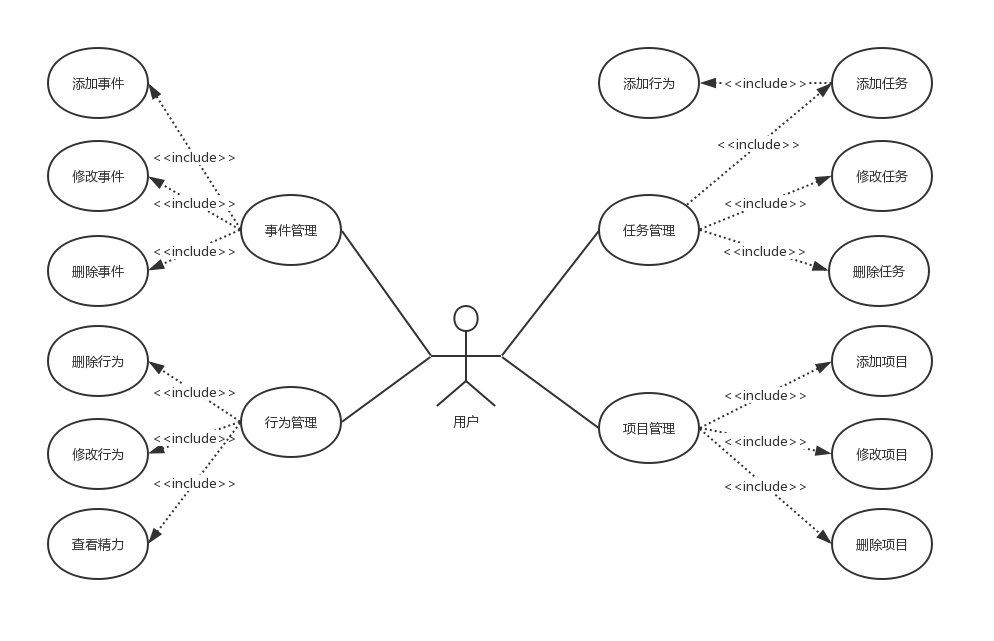
\includegraphics[width=\textwidth]{figure/uml/use_case.png}}
	\caption{任务计划及时间管理系统总用例图}
    \label{fig:use_case}
\end{figure}

图\ref{fig:use_case}基本包含了本系统的所有基本用例,
其中行为管理是根据需求分析得到的用于记录任务完成情况和精力分配的工具,
更为细致的用例描述见以下表格分析。

\begin{table}
	\centering
	\caption{用户添加任务用例描述表}
	\begin{tabular}{l|p{8cm}} \toprule
	  项目 & 内容说明 \\
	  \midrule
	  用例名称 & 用户添加任务 \\
	  参与者 & 用户 \\
	  前提条件 & 无 \\
	  前置操作 & 用户处于主界面状态 \\
	  后置操作 & 用户设置好任务信息后跳转回原界面 \\
	  合法流程 & 用户点击收件箱添加任务或长按收件箱添加任务,
	  设置好任务信息后点击保存 \\
	  异常情况举例 & 数据库或手机内部存储已满,无法添加 \\
	  \bottomrule
	\end{tabular}
\end{table}

\begin{table}
	\centering
	\caption{用户选择任务依赖关系用例描述表}
	\begin{tabular}{l|p{8cm}} \toprule
	  项目 & 内容说明 \\
	  \midrule
	  用例名称 & 用户选择任务依赖关系 \\
	  参与者 & 用户 \\
	  前提条件 & 用户已创建项目且项目中已含有任务 \\
	  前置操作 & 用户添加任务 \\
	  后置操作 & 跳转回添加任务界面 \\
	  合法流程 & 用户点击添加任务,选择合适的项目进行归类,
	  选择同一项目中的其他任务设置依赖关系 \\
	  异常情况举例 & 由于已经通过算法帮助用户排除了可能出现的
	  依赖关系形成环的情况,故在满足前提条件的情况下,基本无异常情况出现 \\
	  \bottomrule
	\end{tabular}
\end{table}

\begin{table}
	\centering
	\caption{用户完成任务用例描述表}
	\begin{tabular}{l|p{8cm}} \toprule
	  项目 & 内容说明 \\
	  \midrule
	  用例名称 & 用户选用户完成任务 \\
	  参与者 & 用户 \\
	  前提条件 & 用户已创建任务 \\
	  前置操作 & 用户添加任务 \\
	  后置操作 & 保持原界面或添加行为界面 \\
	  合法流程 & 用户点击完成任务,若任务未被分割,则直接完成,
	  若任务已被分割,则进入用户添加行为界面 \\
	  异常情况举例 & 数据库或手机内部存储已满,无法添加行为 \\
	  \bottomrule
	\end{tabular}
\end{table}

\begin{table}
	\centering
	\caption{用户添加事件用例描述表}
	\begin{tabular}{l|p{8cm}} \toprule
	  项目 & 内容说明 \\
	  \midrule
	  用例名称 & 用户添加事件 \\
	  参与者 & 用户 \\
	  前提条件 & 用户已授权系统日历使用权限 \\
	  前置操作 & 用户位于今日界面 \\
	  后置操作 & 保持原界面 \\
	  合法流程 & 用户未授权系统日历则弹出对话框授权使用,
	  若已授权则弹出添加事件的界面并进行设置 \\
	  异常情况举例 & 用户未授权系统日历,无法添加事件 \\
	  \bottomrule
	\end{tabular}
\end{table}

对于用户的需求进行分析后,发现任务这一实体的粒度不够细,需要再进行细化
也就是之前提到的行为,通过行为,我们可以更加细腻的了解用户在每个时间段的状态
便于以后的统计和分析,具体如图\ref{fig:activity}。

\begin{figure}
	\centering
	\makebox[\textwidth]{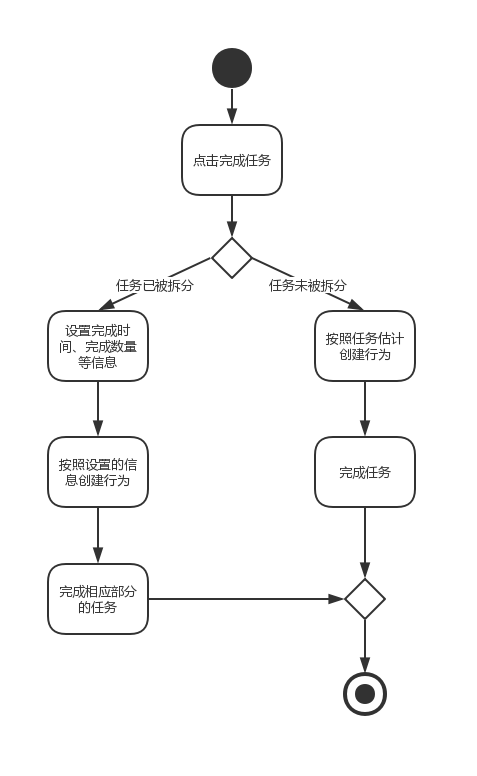
\includegraphics[height=12cm]{figure/uml/activity.png}}
	\caption{用户选择完成任务的活动图}
    \label{fig:activity}
\end{figure}

\section{其他需求}
\subsection{用户界面}
本系统的用户界面采用统一的GUI界面,并保持与iOS 系统应用风格的一致性,
其中出现的所有错误信息和提示信息均采用与系统风格统一的标准提示框。

\subsection{通讯接口}
\begin{itemize}
	\item 预留与Apple 服务器通讯并进行同步的iCloud 服务接口。
	\item 日常使用中可以不依赖网络使用,确保随时可用。
	\item 与其他日程管理类的软件通用接口:如系统日历,iCal通用日历信息文件。
	\item 与其他即时通讯类软件的交互接口:如文字信息入口等。
\end{itemize}

\subsection{性能需求}
\begin{itemize}
	\item 客户端一般响应时间不超过0.1秒。
	\item 任务统计时间不超过0.5秒。
\end{itemize}

\subsection{安全性需求}
\begin{itemize}
	\item 数据备份:允许用户进行数据的备份和恢复,以弥补数据的破坏和丢失。
	\item 加密:可以设置需要指纹或密码进入系统。
\end{itemize}

\subsection{可用性需求}
\begin{itemize}
	\item 控制必录入项:本系统能够对必须录入的内容进行控制,
	确保信息录入的完整。同时对必录入项进行有效的统一的提示,如使保存按钮不可用等。
	\item 容错能力:系统具有一定的容错和抗干扰能力,在非硬件故障或非通讯故障时,
	系统能够保证正常运行,并有足够的提示信息帮助用户有效正确地完成任务。
	\item 对于删除等具有破坏性的操作,提供撤销操作或予以提示。
\end{itemize}
%# -*- coding: utf-8-unix -*-
% !TEX program = xelatex
% !TEX root = ../thesis.tex
% !TEX encoding = UTF-8 Unicode
\chapter{系统设计}
完成系统的定义阶段之后,便进入了系统的设计阶段,
主要完成对系统的结构设计、系统模块设计与数据库表结构设计。
\section{系统框架结构设计}
本系统为满足不依赖网络、随时可用和安全性的特点,采用单用户体系结构,
本框架是我在iOS已有框架(Core Data和Event Kit)
的基础上融合而来,这两个框架都和Apple的服务紧密结合,方便今后对其进行扩展。
基本框架结构如图\ref{fig:level}所示。

\begin{figure}[!htbp]
	\centering
	\makebox[\textwidth]{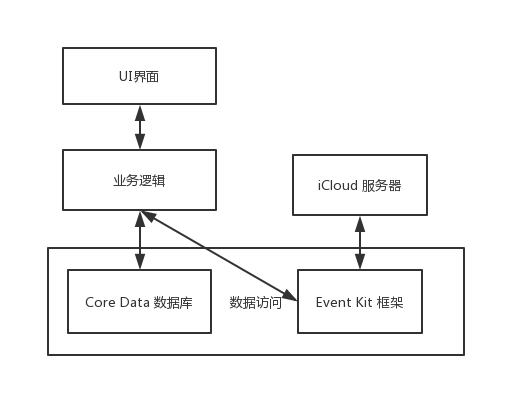
\includegraphics[height=8cm]{figure/level.png}}
	\caption{系统框架结构示意图}
    \label{fig:level}
\end{figure}

Core Data 是Apple提供的持久化数据的方案,一般来说,底层使用的是 Sqlite 数据库,如图\ref{fig:core_data}所示。
\begin{figure}[!htbp]
	\centering
	\makebox[\textwidth]{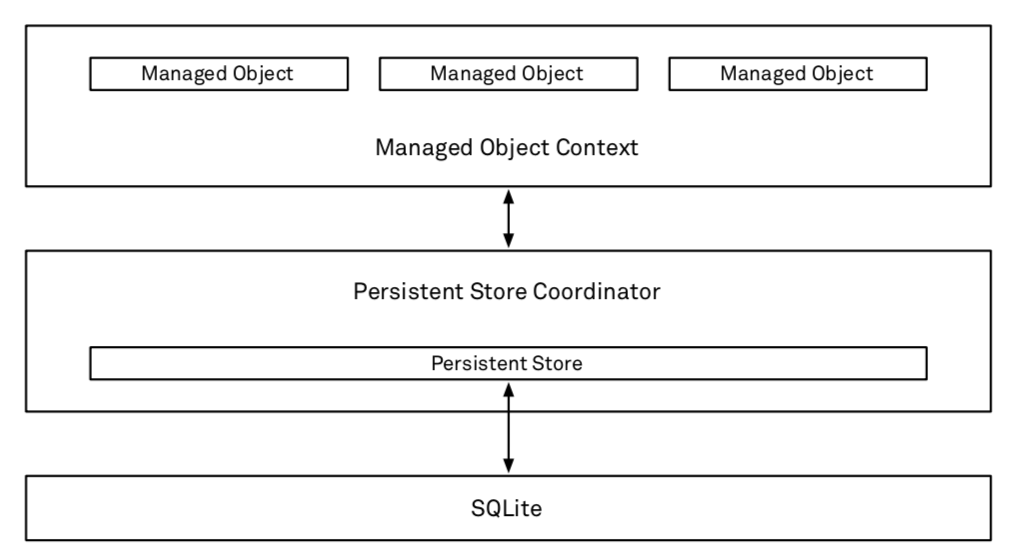
\includegraphics[height=6cm]{figure/core_data.png}}
	\caption{Core Data 结构示意图}
    \label{fig:core_data}
\end{figure}

\section{系统模块设计}
为保证系统的可拓展性和开发的便利,将系统分解为几个主要模块,如图\ref{fig:part}。
\begin{figure}[!htbp]
	\centering
	\makebox[\textwidth]{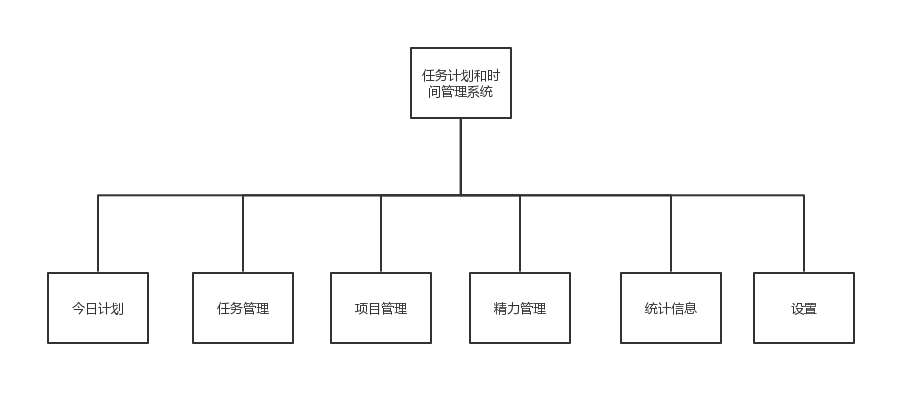
\includegraphics[width=\textwidth]{figure/part.png}}
	\caption{系统模块结构图}
    \label{fig:part}
\end{figure}

从图中可以看出任务计划及时间管理系统的架构设计,可以分为六个模块,
今日计划模块、任务管理模块、项目管理模块、精力管理模块、统计信息模块、设置模块,
系统通过用户输入获取信息,将信息保存到本地的数据库或系统的EventKit中,
再通过业务逻辑将信息经过排序、筛选等处理后进行展示。
其中每个模块均可直接通过主界面到达,将系统拆分为各个模块后,
降低了系统的耦合性,增强了系统的可拓展性。

\section{数据库设计}

\subsection{系统实体关系图}
由于Core Data会通过数据表之间的概念数据模型和他们之间的关系生成相应的物理模型(包括ID和主外建等),
无需开发者生成具体的物理模型。
图\ref{fig:e-r}中出现的事件和日历均为iOS系统自带的实体,也无需保存入Core Data 数据库中。
Core Data中的数据实体如图\ref{fig:core-data}所示。
\begin{figure}[!htbp]
	\centering
	\makebox[\textwidth]{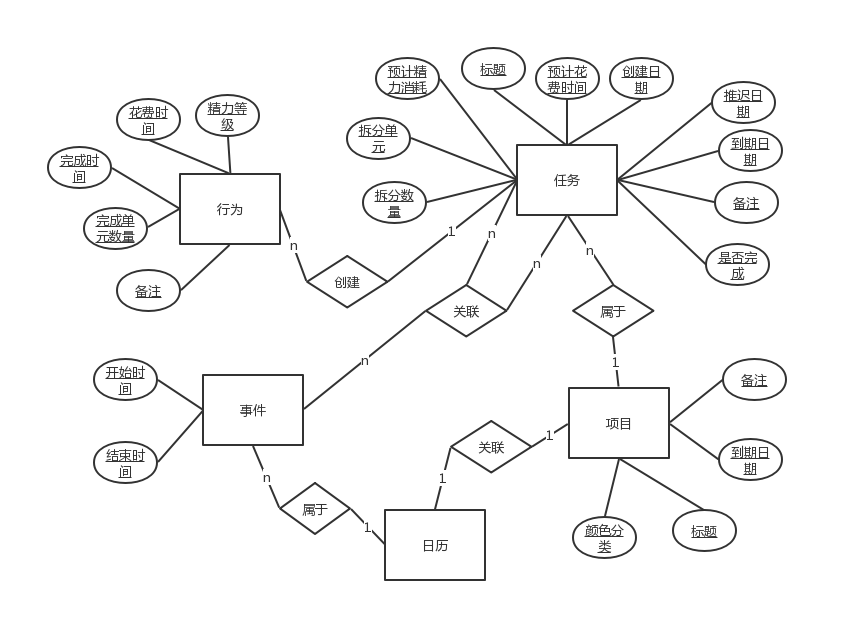
\includegraphics[width=\textwidth]{figure/e-r.png}}
	\caption{实体关系图}
    \label{fig:e-r}
\end{figure}

\begin{figure}[!htbp]
	\centering
	\makebox[\textwidth]{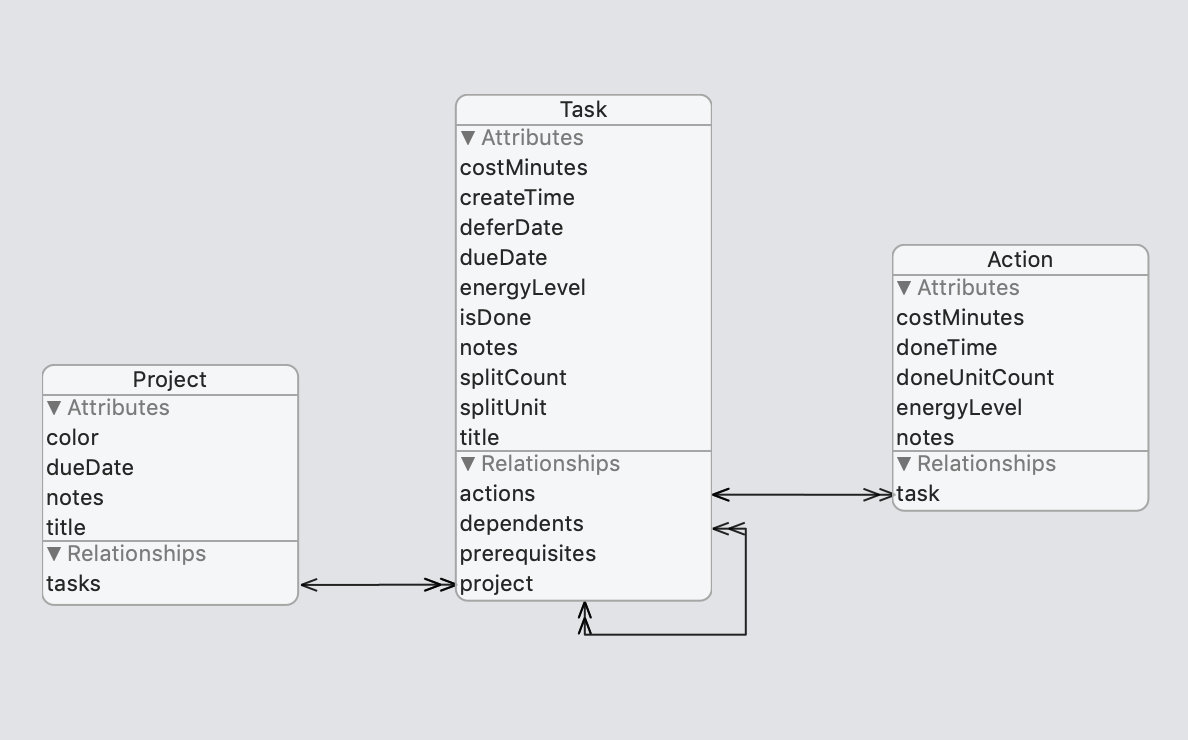
\includegraphics[width=\textwidth]{figure/relationship.png}}
	\caption{Core Data 数据实体及关系图}
	\label{fig:core-data}
\end{figure}

\subsection{系统数据表}

\begin{table}[H]
  \centering
  \caption{任务表}
  \begin{tabular}{ccccccc} \toprule
	序号 & 列名 & 数据类型 & 允许空 & 说明 & 备注 \\
	\midrule
	1 & costMinutes & Integer32 & 否 & 花费时间 & 无 \\
	2 & createTime & Date & 否 & 创建时间 & 无 \\
	3 & deferDate & Date & 否 & 推迟日期 & 无 \\
	4 & dueDate & Date & 否 & 到期时间 & 无 \\
	5 & energyLevel & Integer16 & 否 & 精力等级 & 无 \\
	6 & isDone & Boolean & 否 & 是否完成 & 无 \\
	7 & notes & String & 否 & 备注 & 无 \\
	8 & splitCount & Integer32 & 否 & 拆分数量 & 无 \\
	9 & splitUnit & String & 否 & 拆分单位 & 无 \\
	10 & title & String & 否 & 标题 & 无 \\
	\bottomrule
  \end{tabular}
\end{table}

\begin{table}[H]
	\centering
	\caption{项目表}
	\begin{tabular}{ccccccc} \toprule
	  序号 & 列名 & 数据类型 & 允许空 & 说明 & 备注 \\
	  \midrule
	  1 & color & Transformable & 否 & 花费时间 & UIColor \\
	  2 & dueDate & Date & 否 & 到期时间 & 无 \\
	  3 & notes & String & 否 & 备注 & 无 \\
	  4 & title & String & 否 & 题目 & 无 \\
	  \bottomrule
	\end{tabular}
\end{table}

\begin{table}[H]
	\centering
	\caption{行为表}
	\begin{tabular}{ccccccc} \toprule
	  序号 & 列名 & 数据类型 & 允许空 & 说明 & 备注 \\
	  \midrule
	  1 & costMinutes & Integer32 & 否 & 花费时间 & UIColor \\
	  2 & doneTime & Date & 否 & 完成时间 & 无 \\
	  3 & doneUnitCount & Integer32 & 否 & 完成数量 & 无 \\
	  4 & energyLevel & Integer16 & 否 & 精力花费 & 无 \\
	  5 & notes & String & 否 & 备注 & 无 \\
	  \bottomrule
	\end{tabular}
\end{table}


%# -*- coding: utf-8-unix -*-
% !TEX program = xelatex
% !TEX root = ../thesis.tex
% !TEX encoding = UTF-8 Unicode

\chapter{系统实现}

在前两个章节中,已经进行了系统的需求分析并明确了系统设计的方法,
本章将按照前文所确定的需求和设计,利用软件开发工具和相关技术完成
基于iOS的任务计划及时间管理系统

\section{系统的实现环境}
本系统开发采用的IDE为 Xcode,数据库为Core Data,主要开发语言为 Swift。
由于本系统采用的Swift版本为Swift 5 故需要iOS 8.0以上的操作系统才可以使用,
考虑到iOS新版本的普及率,是可以接受的。

\section{系统模块的实现}
本程序主要涉及事件管理、项目管理、任务管理、精力分析、行为管理五个模块,
每个模块都有众多功能,以下仅对这五个模块中的主要功能的实现进行介绍。

\subsection{事件管理模块}
根据系统设计阶段的需求,事件管理模块应能正确访问系统自带的日历
并能对其中的事件进行添加、删除和修改,并将相关的数据保存到系统的EventStore中,
以实现系统自身基于iCloud的同步。在初次进入主界面时,请求对系统日历的读写权限,
若已经授权则在后台读取今天的日程并进行展示,不影响主线程的操作,同时提供添加日程和编辑日程的功能。

由于用户可能随时关闭对该应用对日历的访问权限,故每次都需要对日历权限进行检查,若没有授权则进行请求。
具体代码和效果图如下。

\begin{lstlisting}[language={Swift}, caption={请求日历权限代码逻辑}]
	func checkEventAuthorizationStatus() {
		let status = EKEventStore.authorizationStatus(for: .event)
		switch status {
		case .notDetermined:
			requestAccessToEvent()
		case .authorized:
			break
		default:
			break
		}
	}
	func requestAccessToEvent() {
		store.requestAccess(to: EKEntityType.event, completion: {
			(accessGranted: Bool, error: Error?) in
			if accessGranted == true {
				DispatchQueue.main.async(execute: {
					// ...
				})
			}
		})
	}
\end{lstlisting}

\begin{figure}[H]
	\centering
	\makebox[\textwidth]{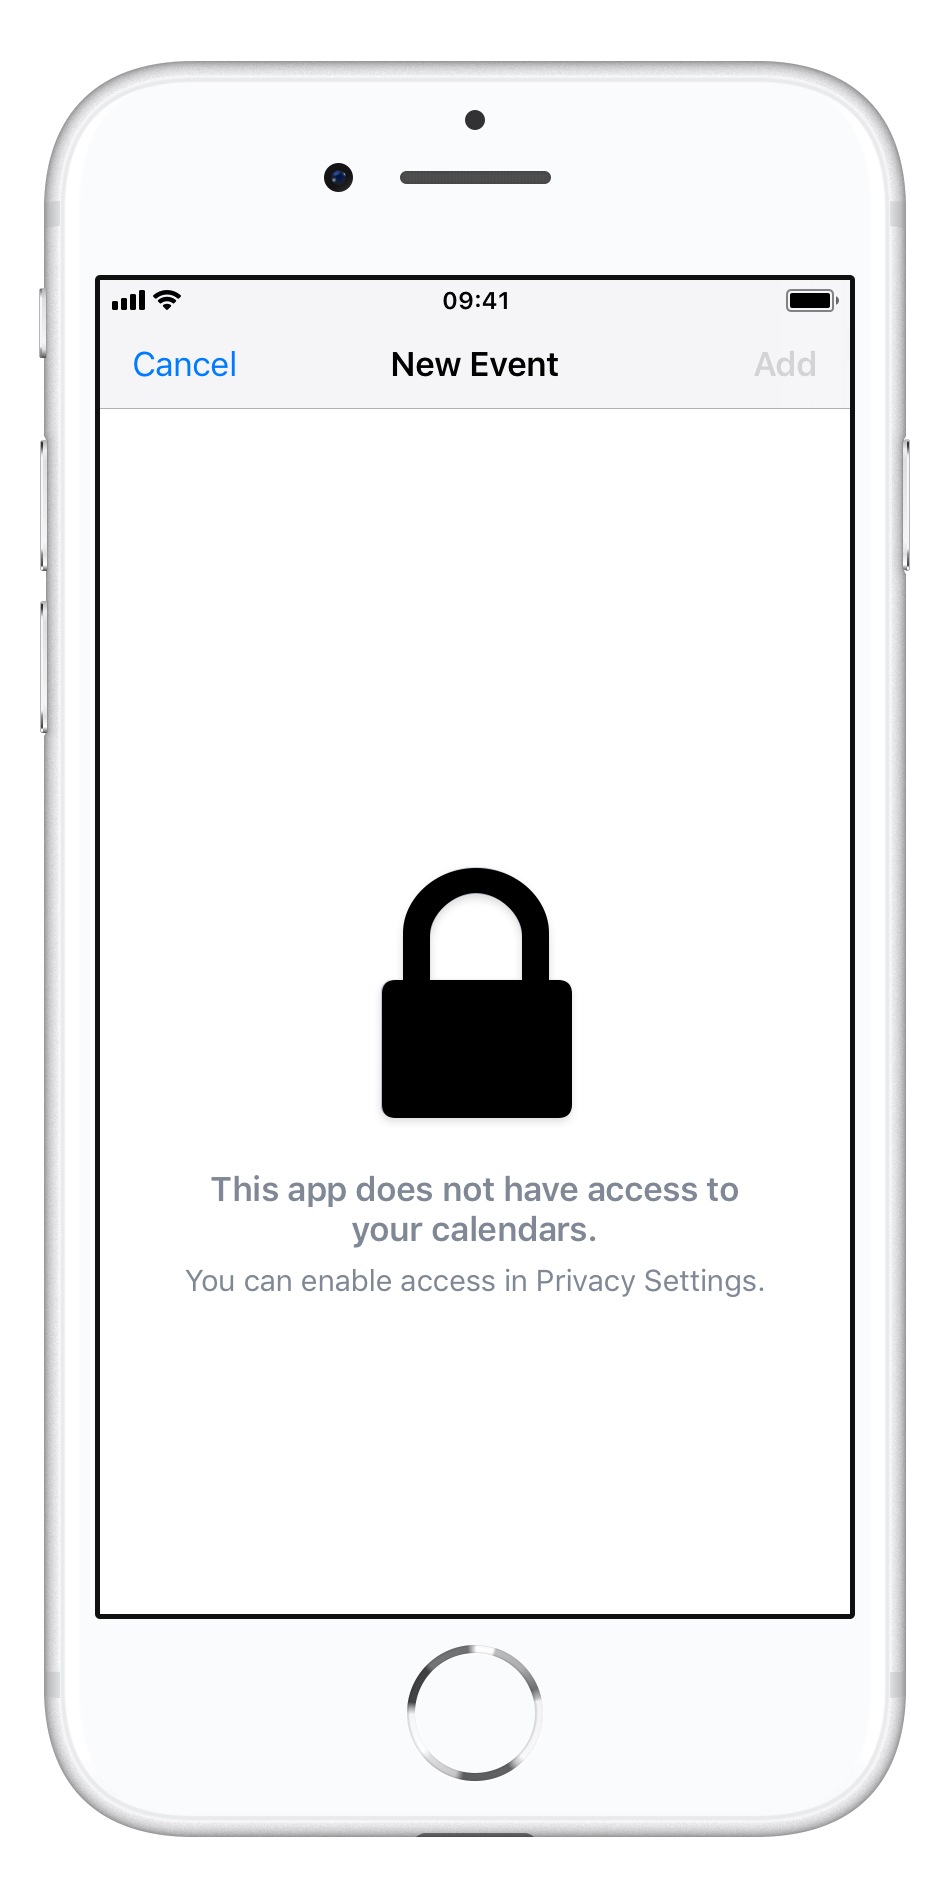
\includegraphics[height=10cm]{figure/system/new_event+no_access}}
	\caption{未获取日历权限创建新事件截图}
\end{figure}

\begin{figure}[H]
	\centering
	\makebox[\textwidth]{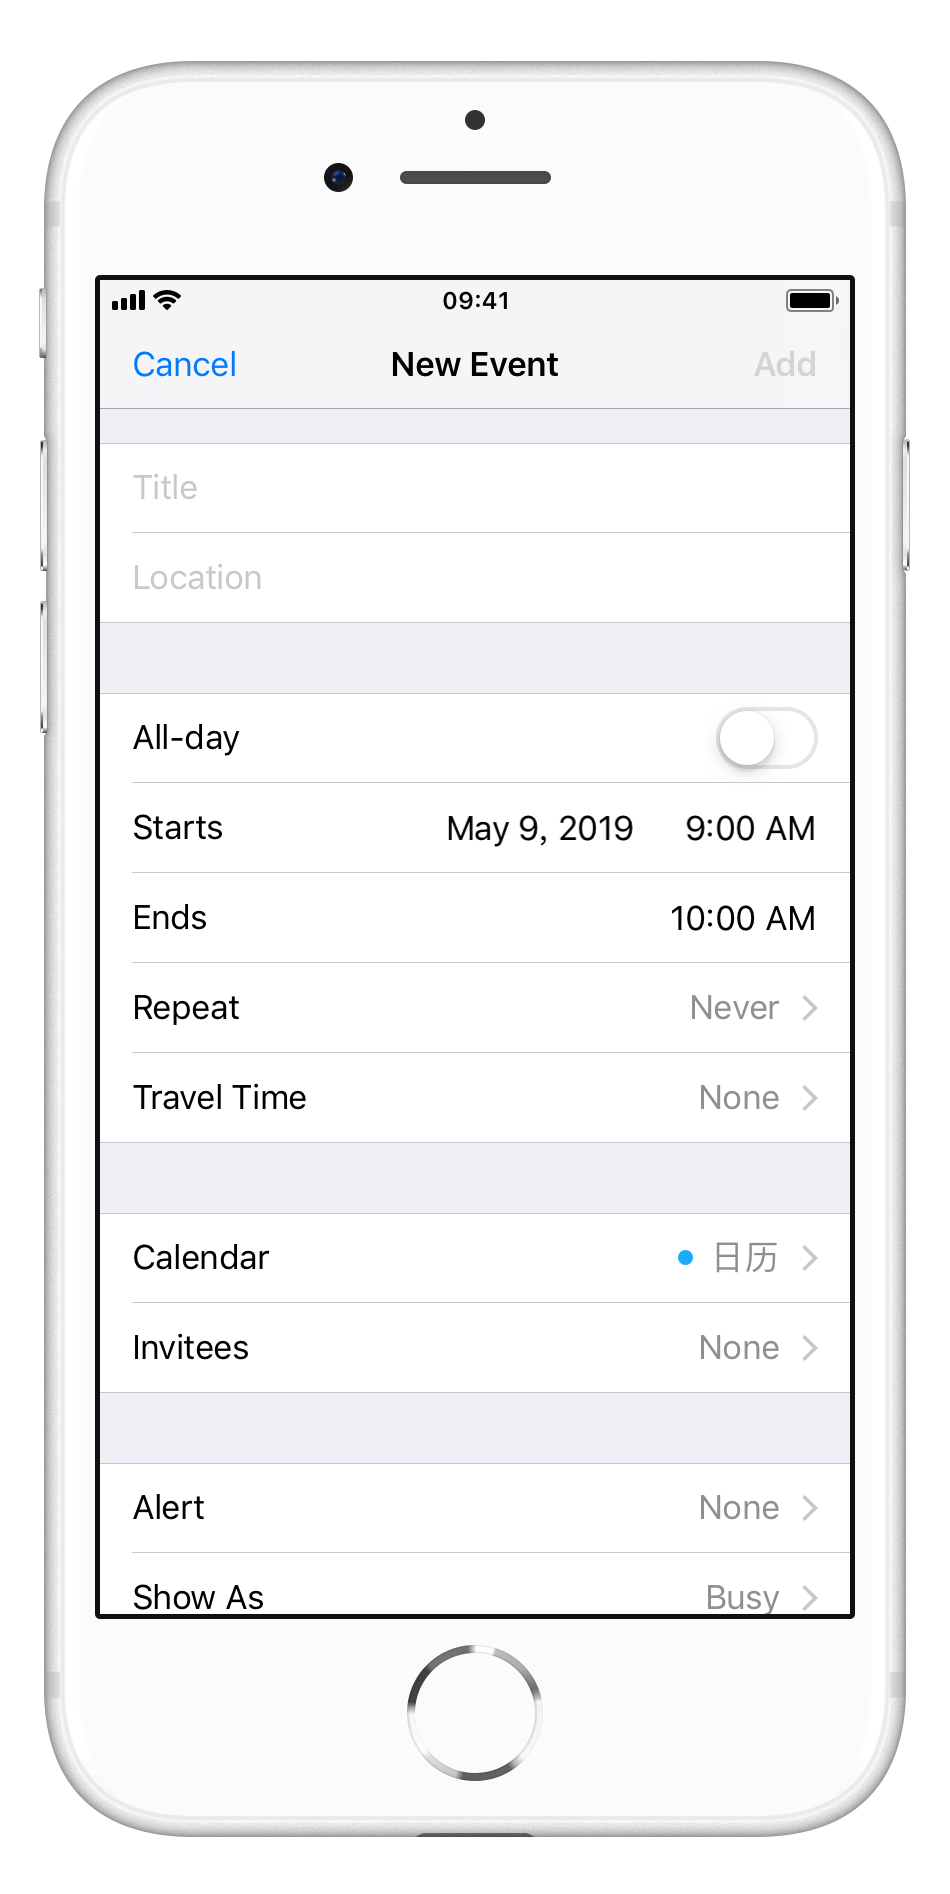
\includegraphics[height=10cm]{figure/system/new_event}}
	\caption{已获取日历权限创建新事件截图}
\end{figure}

\subsection{任务管理模块}
用户可以添加任务、修改任务、删除任务或将任务标记为已完成,
在Inbox(收件箱)\footnote{此处的收件箱并不是指邮件系统的收件箱,而是GTD理念中的将待办事项整合起来的地方。}
中,用户可以通过系统自带Siri功能\footnote{目前采用的是一种曲线救国的方法,即通过EventKit访问系统自带的提醒事项来达到类似Siri直接添加的效果。}
无需说应用名称,就可以添加新任务,这大大减少了输入带来的不便。
具体代码如下。

\begin{lstlisting}[language={Swift}, caption={请求提醒事项权限并导入系统代码逻辑}]
	func checkReminderAuthorizationStatus() {
        let status = EKEventStore.authorizationStatus(for: .reminder)
        switch status {
        case .notDetermined:
            requestAccessToReminder()
        case .authorized:
            loadReminders()
        default:
            break
        }
    }
    
    func requestAccessToReminder() {
        store.requestAccess(to: EKEntityType.reminder, completion: {
            (accessGranted: Bool, error: Error?) in
            
            if accessGranted == true {
                DispatchQueue.main.async(execute: {
                    self.loadReminders()
                    self.updateTasks()
                })
            }
        })
    }
    
    func loadReminders() {
        let predicate: NSPredicate? = store.predicateForReminders(in: [store.defaultCalendarForNewReminders()!])
        if let aPredicate = predicate {
            store.fetchReminders(matching: aPredicate, completion: {(_ reminders: [EKReminder]?) -> Void in
                for reminder: EKReminder? in reminders ?? [EKReminder?]() {
                    if(!reminder!.isCompleted) {
                        let task = Task(context: self.context)
                        task.title = reminder?.title
                        task.notes = reminder?.notes
                        task.dueDate = reminder?.dueDateComponents?.date
                        try? self.store.remove(reminder!, commit: true)
                        try? self.context.save()
                    }
                }
            })
        }
    }
    func updateTasks() {
        let request: NSFetchRequest<Task> = Task.fetchRequest()
        let predicate = NSPredicate(format: "project == %@", sourceProject ?? 0)
        request.predicate = predicate
        tasks = try! context.fetch(request)
    }
\end{lstlisting}

这项功能只会导入系统提醒事项中未完成的任务,避免数据过多导致缺失重点。

\begin{figure}[H]
	\centering
	\makebox[\textwidth]{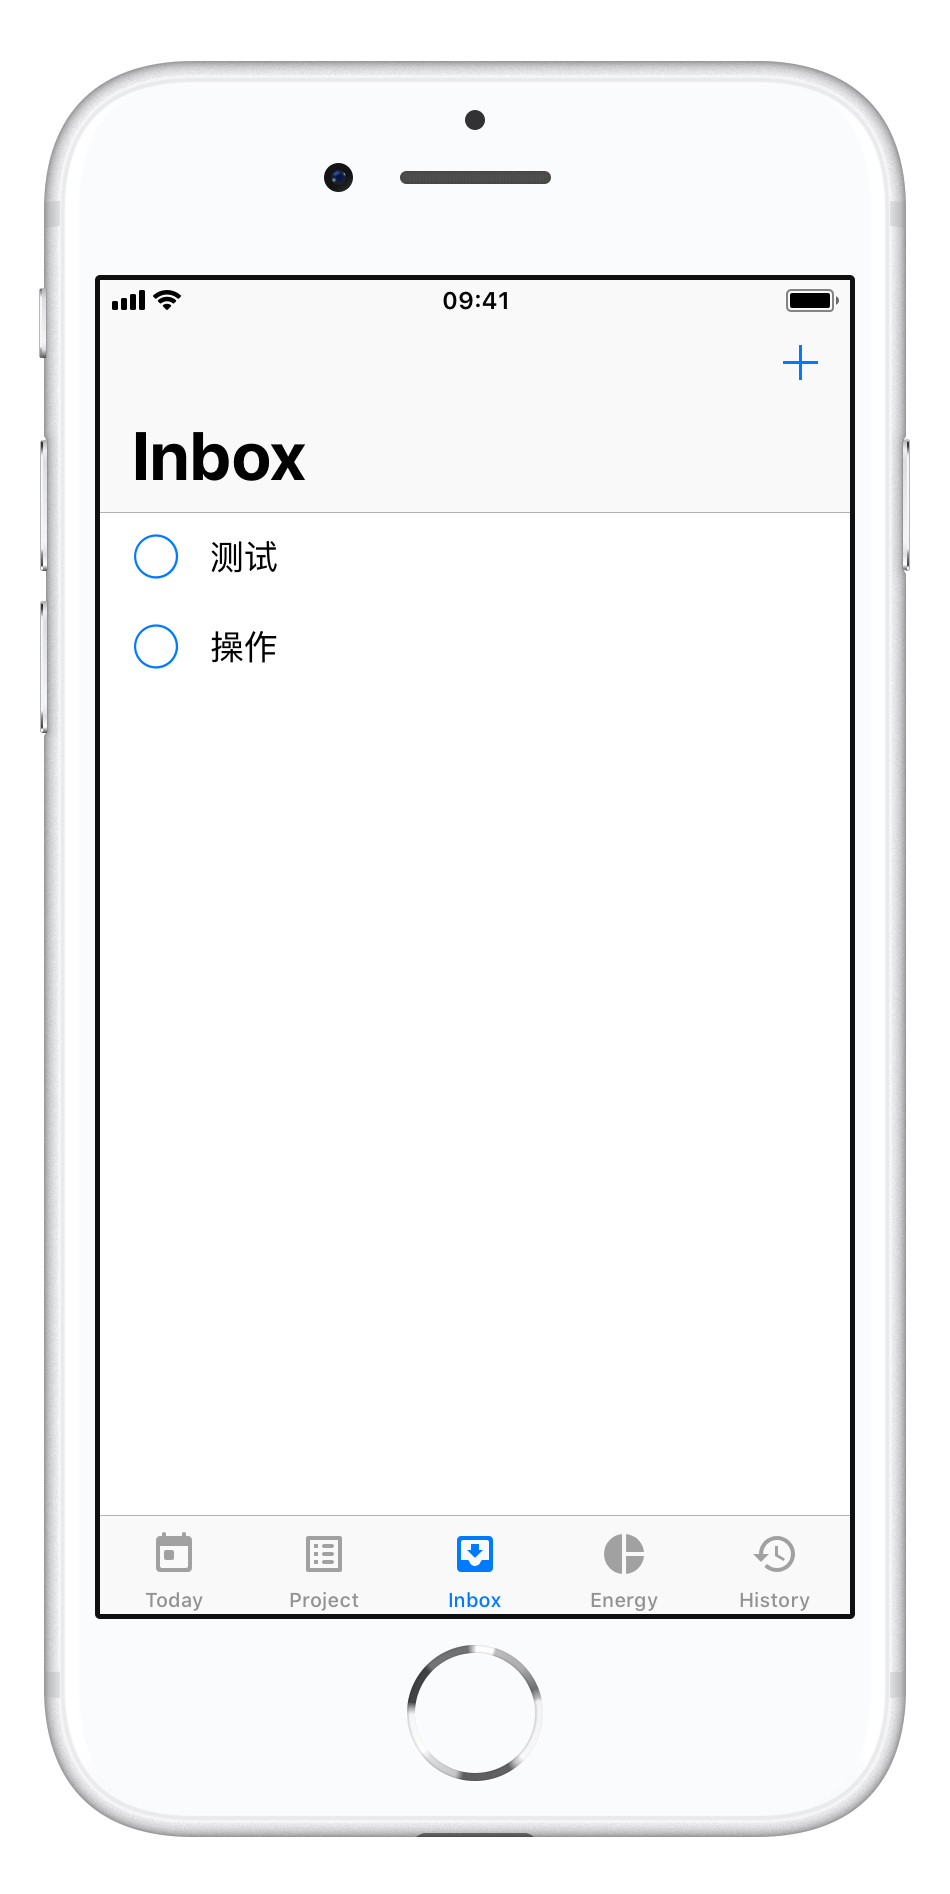
\includegraphics[height=10cm]{figure/system/inbox+no_split}}
	\caption{从系统提醒事项中拉取任务截图}
\end{figure}

对于任务是否完成,通过任务TableViewCell中左侧的图标来进行提示,并可以通过点击图标将任务标记为已完成,
根据MVC设计的原则由于TableViewCell本身并不了解任务的相关属性,自然也无从得知用户点击了哪一个任务的完成图标,
故需要通过代理告知TableViewController,由后者完成任务完成的相关操作。

\begin{lstlisting}[language={Swift}, caption={TaskTableViewCell}]
	@objc protocol TaskCellDelegate: class {
		func checkMarkTapped(sender: TaskTableViewCell)
	}

	class TaskTableViewCell: UITableViewCell {
		
		var delegate: TaskCellDelegate?
		
		@IBOutlet weak var doneProgressView: UIProgressView!
		
		@objc func imageViewTapped() {
			delegate?.checkMarkTapped(sender: self)
		}
		
		func update(with task: Task) {
			let color = task.project?.color as? UIColor
			textLabel?.text = task.title
			imageView?.image = task.isDone ? UIImage(named: "dot circle") : UIImage(named: "circle")
			imageView?.tintColor = color
			doneProgressView.isHidden = task.splitCount == 1
			doneProgressView.progressTintColor = color
			doneProgressView.trackTintColor = color?.withAlphaComponent(0.1)
		}
		
		override func awakeFromNib() {
			super.awakeFromNib()
			let leadingConstraint = NSLayoutConstraint.init(item: doneProgressView!, attribute: .leading, relatedBy: .equal, toItem: textLabel, attribute: .leading, multiplier: 1.0, constant: 0)
			self.addConstraints([leadingConstraint])
			imageView?.isUserInteractionEnabled = true
			let gesture = UITapGestureRecognizer(target: self, action: #selector(imageViewTapped))
			gesture.numberOfTapsRequired = 1
			imageView?.addGestureRecognizer(gesture)
		}
	}
\end{lstlisting}

\begin{lstlisting}[language={Swift}, caption={TaskListTableViewController实现代理的相关代码}]
	class TaskListTableViewController: UITableViewController, TaskCellDelegate {
		let context = AppDelegate.viewContext
		var store = EKEventStore()
		var tasks = [Task]()
		var sourceProject: Project? = nil
		...
		func checkMarkTapped(sender: TaskTableViewCell) {
        if let indexPath = tableView.indexPath(for: sender) {
            let task = tasks[indexPath.row]
            if task.splitCount == 1 {
                task.isDone = !task.isDone
                let action = Action(context: context)
                action.costMinutes = task.costMinutes
                action.doneTime = Date()
                action.doneUnitCount = 1
                action.energyLevel = task.energyLevel
                action.task = task
                try! context.save()
            }
            else {
                let sb = UIStoryboard(name: "Main", bundle: nil)
                let navViewController = sb.instantiateViewController(withIdentifier: "navAEAction") as! UINavigationController
                let vc = navViewController.topViewController as? AddEditActionTableViewController
                vc?.task = task
                present(navViewController, animated: true, completion: nil)
            }
            tasks[indexPath.row] = task
            tableView.reloadRows(at: [indexPath], with: .automatic)
		}
		...
    }
\end{lstlisting}

本系统的主要功能在于对任务进行详尽的设置,并通过相关的设置,对用户的任务完成情况,行为等进行跟踪和分析。
为了方便用户的设置,本系统尽可能的减少了用户的输入操作,改用DatePicker等便于输入的方式进行添加任务。

\begin{figure}[H]
	\centering
	\makebox[\textwidth]{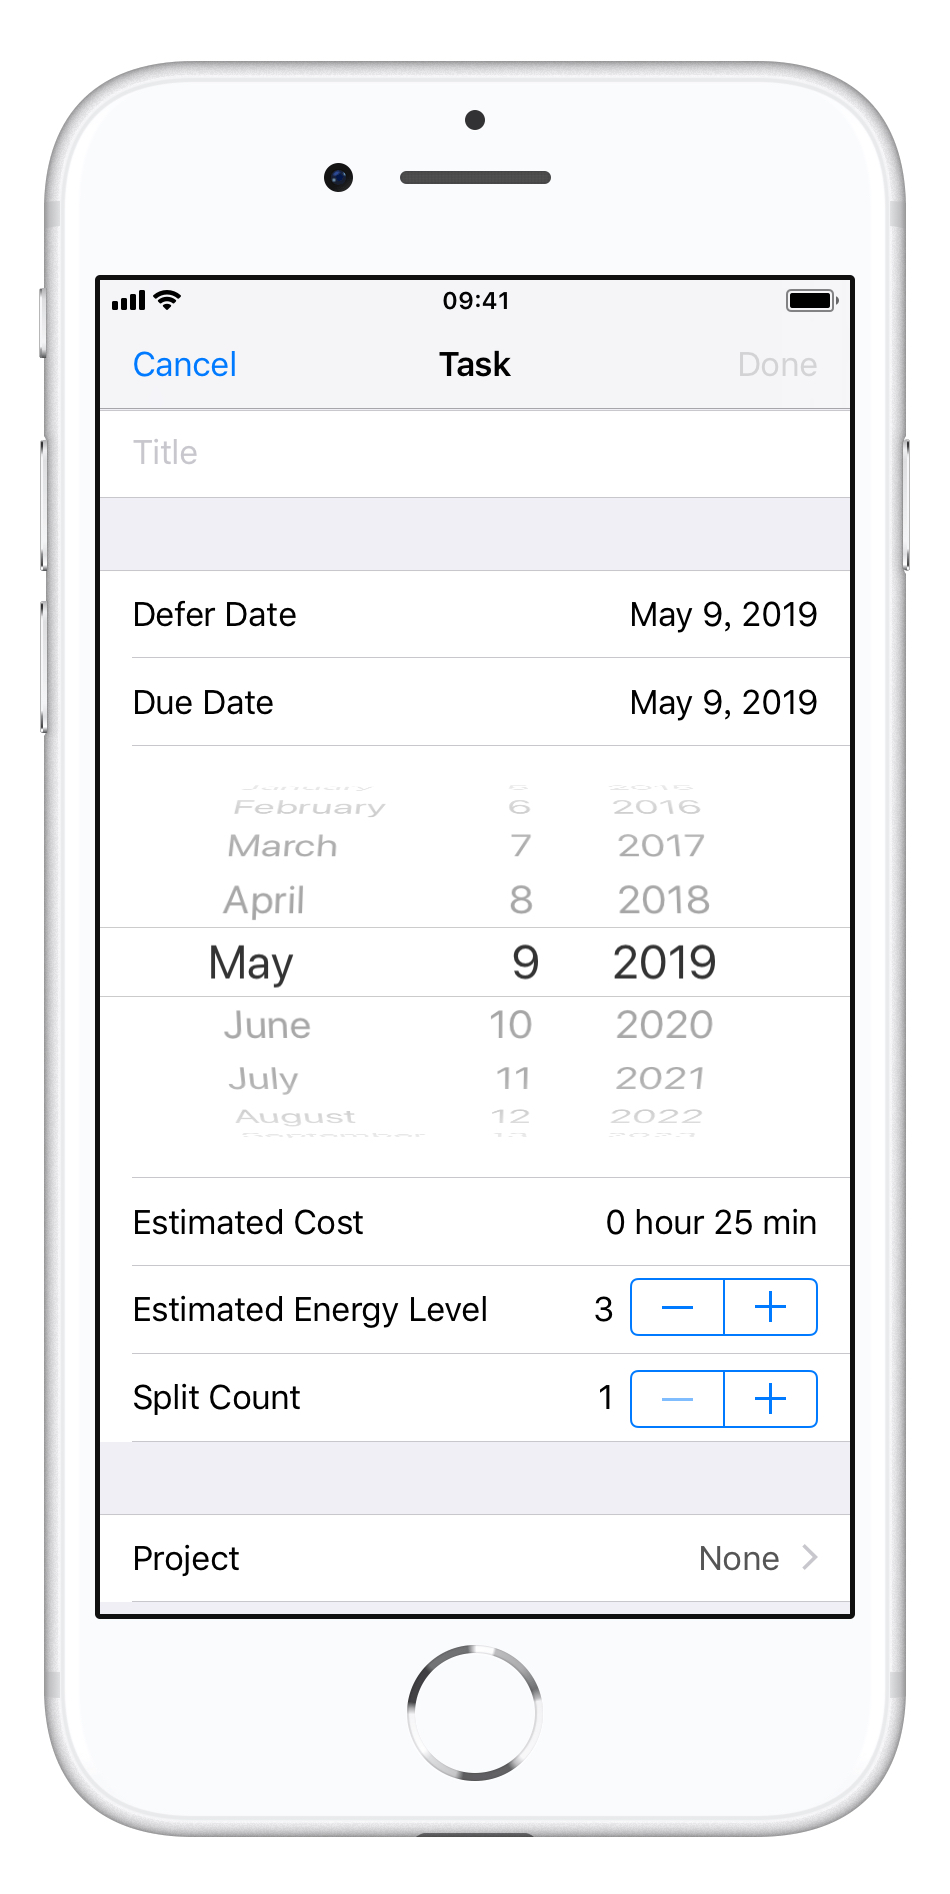
\includegraphics[height=10cm]{figure/system/add_task+duedate}}
	\caption{使用DatePicker添加到期日期}
\end{figure}

对于多个日期和表单的情况,通过代码动态控制TableView的行高来实现不同DatePicker的切换,代码如下。

\begin{lstlisting}[language={Swift}, caption={动态调整行高以便输入}]
	...
	let deferDatePickerCellIndexPath = IndexPath(row: 1, section: 1)
    let dueDatePickerCellIndexPath = IndexPath(row: 3, section: 1)
    let costTimePickerCellIndexPath = IndexPath(row: 5, section: 1)
    let splitUnitCellIndexPath = IndexPath(row: 8, section: 1)
    let projectCellIndexPath = IndexPath(row: 0, section: 2)
    let notesTextViewIndexPath = IndexPath(row: 0, section: 3)
    var isDeferDatePickerShown: Bool = false {
        didSet {
            deferDatePicker.isHidden = !isDeferDatePickerShown
        }
    }
    var isDueDatePickerShown: Bool = false {
        didSet {
            dueDatePicker.isHidden = !isDueDatePickerShown
        }
    }
    var isDurationTimePickerShown: Bool = false {
        didSet {
            costTimePicker.isHidden = !isDurationTimePickerShown
        }
    }
	...
	override func tableView(_ tableView: UITableView, didSelectRowAt indexPath: IndexPath) {
        tableView.deselectRow(at: indexPath, animated: true)
        view.endEditing(true)   // Hide Keyboard
        // Toggle DatePicker
        switch (indexPath.section, indexPath.row) {
        case (deferDatePickerCellIndexPath.section, deferDatePickerCellIndexPath.row - 1):
            isDeferDatePickerShown = !isDeferDatePickerShown
            isDueDatePickerShown = false
            isDurationTimePickerShown = false
            updateTableView()
            
        case (dueDatePickerCellIndexPath.section, dueDatePickerCellIndexPath.row - 1):
            isDeferDatePickerShown = false
            isDueDatePickerShown = !isDueDatePickerShown
            isDurationTimePickerShown = false
            updateTableView()
            
        case (costTimePickerCellIndexPath.section, costTimePickerCellIndexPath.row - 1):
            isDeferDatePickerShown = false
            isDueDatePickerShown = false
            isDurationTimePickerShown = !isDurationTimePickerShown
            updateTableView()
        
        default:
            break
        }
	}
	
	override func tableView(_ tableView: UITableView, heightForRowAt indexPath: IndexPath) -> CGFloat {
        // Define Date Picker height
        switch (indexPath) {
        case deferDatePickerCellIndexPath:
            return isDeferDatePickerShown ? 216.0 : 0.0
        
        case dueDatePickerCellIndexPath:
            return isDueDatePickerShown ? 216.0 : 0.0
        
        case costTimePickerCellIndexPath:
            return isDurationTimePickerShown ? 216.0 : 0.0
        
        case splitUnitCellIndexPath:
            return isSplitEnable ? 44.0 : 0.0
            
        case [projectCellIndexPath.section, projectCellIndexPath.row + 1],
             [projectCellIndexPath.section, projectCellIndexPath.row + 2]:
            return isProjectSelected ? 44.0 : 0.0
            
        case (notesTextViewIndexPath):
            return 180.0
        
        default:
            return 44.0
        }
    }
\end{lstlisting}

\subsection{项目管理模块}
项目管理的一个重要功能是能够选择项目中任务之间的依赖,
实现这一需求的解决方案是通过建立数据库中任务表到自身的关系。
并通过算法计算任务的所有依赖和所有后续,从而避免用户在选择依赖任务或后续任务时形成依赖环路。

\begin{lstlisting}[language={Swift}, caption={计算任务依赖关系的代码}]
	extension Task {
		func getAllPrerequisites() -> Set<Task> {
			let selfPrerequisites = self.prerequisites as! Set<Task>
			if selfPrerequisites.isEmpty {
				return []
			} else {
				var childPrerequisites = Set<Task>()
				for prerequisite in selfPrerequisites {
					for task in prerequisite.getAllPrerequisites() {
						childPrerequisites.insert(task)
					}
				}
				return childPrerequisites.union(selfPrerequisites)
			}
		}
		
		func getAllDependents() -> Set<Task> {
			let selfDependents = self.dependents as! Set<Task>
			if selfDependents.isEmpty {
				return []
			} else {
				var childDependents = Set<Task>()
				for dependent in selfDependents {
					for task in dependent.getAllPrerequisites() {
						childDependents.insert(task)
					}
				}
				return childDependents.union(selfDependents)
			}
		}
	}
\end{lstlisting}

extension 是Swift中的一个语言特性,可以在不接触类源代码的情况下为类添加方法和计算属性。
由于本系统直接使用Core Data根据数据库的属性和表以及实体间的关系自动生成相关的类,且在Xcode中
默认并不可见,故使用extension 是比较方便和合适的做法。

\begin{figure}[H]
	\centering
	\makebox[\textwidth]{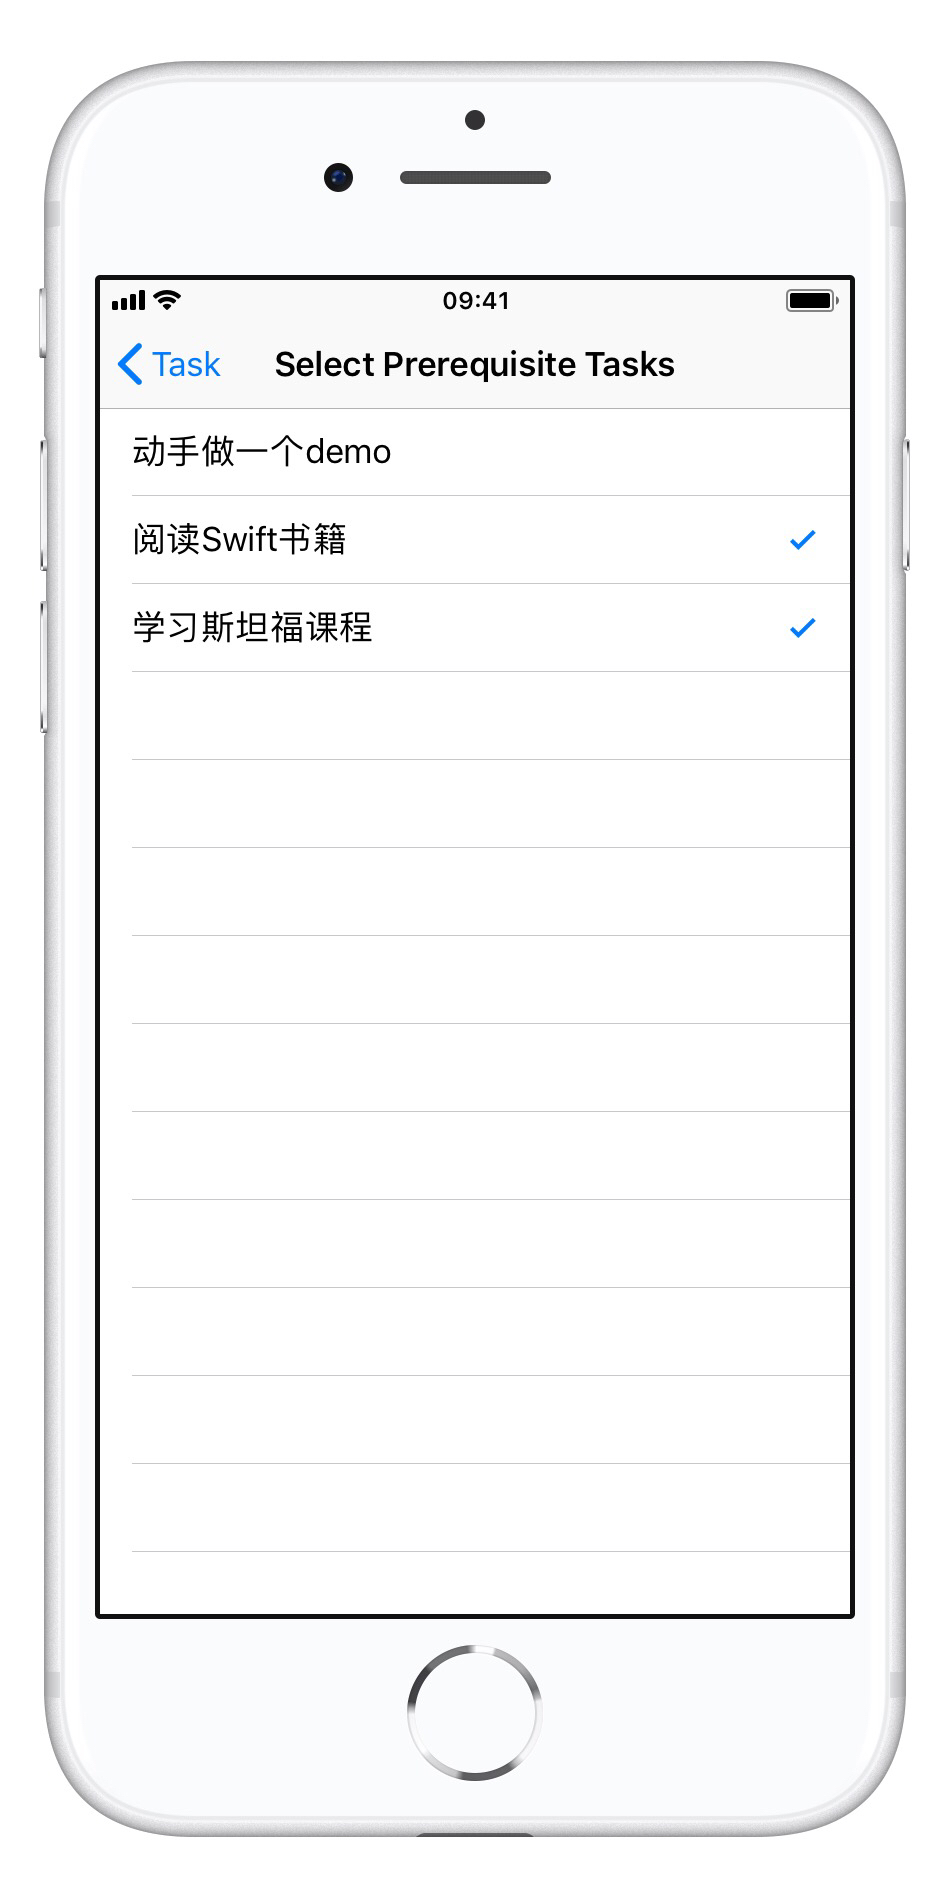
\includegraphics[height=10cm]{figure/system/select_prerequisites_tasks}}
	\caption{选择依赖任务}
\end{figure}

为了实现代码和视图的重用,采用标示信息区别用户选择的任务性质。

\begin{lstlisting}[language={Swift}, caption={选择任务界面的代码}]
class SelectTaskTableViewController: UITableViewController {

    let context = AppDelegate.viewContext
    var tasks = [Task]()
    var selectedTasks = [Task]()
    var identifier = ""
    
    override func viewWillDisappear(_ animated: Bool) {
        if isMovingFromParent {
            let navController = parent as! UINavigationController
            let addEditTaskTableViewController = navController.topViewController as! AddEditTaskTableViewController
            selectedTasks = []
            for i in 0..<tasks.count {
                let cell = tableView.cellForRow(at: [0,i])
                if cell?.accessoryType == .checkmark {
                    selectedTasks.append(tasks[i])
                }
            }
            switch identifier {
            case "SelectDependentTasks":
                addEditTaskTableViewController.dependentsTasks = selectedTasks
            case "SelectPrerequisiteTasks":
                addEditTaskTableViewController.prerequisiteTasks = selectedTasks
            default:
                break
            }
        }
    }
}
\end{lstlisting}

\subsection{精力管理模块}
\begin{figure}[H]
	\centering
	\makebox[\textwidth]{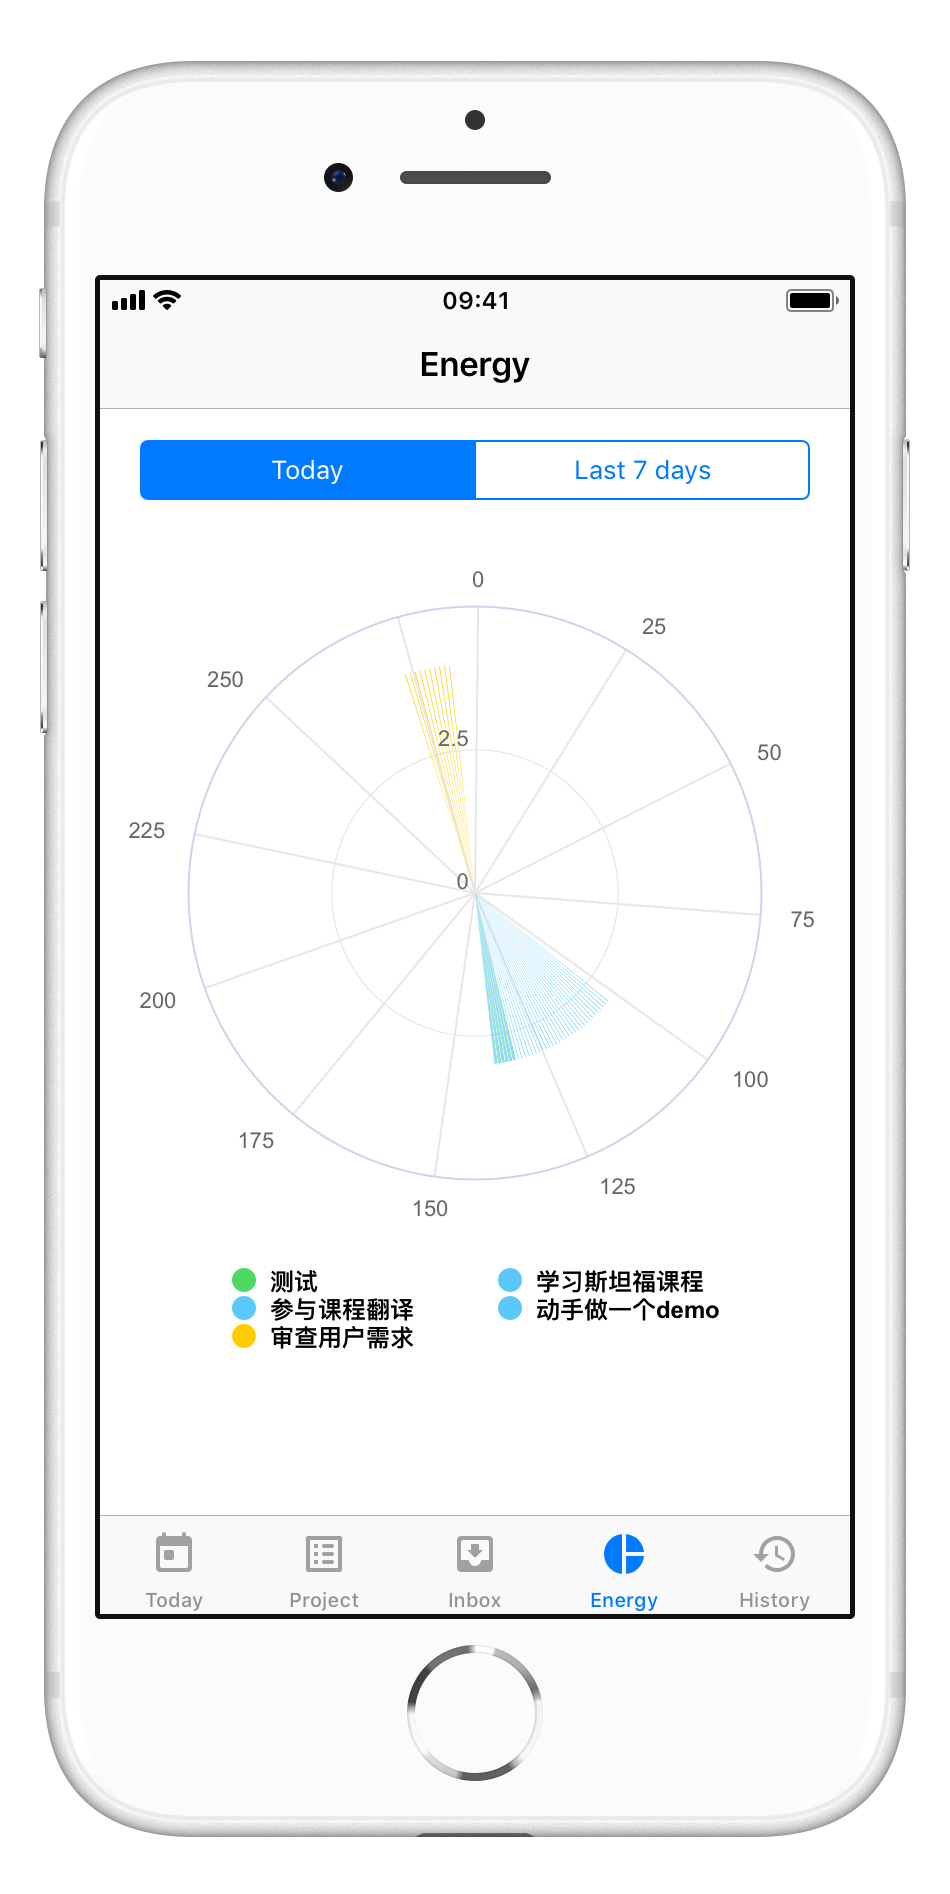
\includegraphics[height=10cm]{figure/system/energy}}
	\caption{查看精力极地图}
\end{figure}
本模块采用第三方库 AAChartView 相关代码如下。
通过对行为完成时间的计算,以5分钟为间隔绘制相应时间段的用户精力情况。

\begin{lstlisting}[language={Swift}, caption={绘制极地图的代码}]
var aaChartModel = AAChartModel()
	.chartType(chartType!)//图形类型
	.polar(true)
	.title("")
	.dataLabelEnabled(false)//是否显示数字
	.animationType(.bounce)//图形渲染动画类型为"bounce"

var chartModelData = [[String : Any]]()

var taskSet = Set<Task>()
for action in actions {
	taskSet.insert(action.task!)
}

for task in taskSet {
	var data = Array(repeating: 0, count: 24*60/5)
	let actions = task.actions as? Set<Action>
	let calendar = Calendar.current
	for action in actions! {
		let dateComponents = calendar.dateComponents(in: calendar.timeZone, from: action.doneTime!)
		let end = (dateComponents.hour! * 60 + dateComponents.minute!) / 5
		let begin = end - Int(action.costMinutes/5)
		for i in begin...end {
			data[i] = Int(action.energyLevel)
		}
	}
	let color = task.project?.color as? UIColor
	let element = AASeriesElement()
	element.name(task.title!)
	element.color(color!.hexString!)
	element.data(data)
	chartModelData.append(element.toDic()!)
}

aaChartModel = aaChartModel.series(chartModelData)

aaChartView?.aa_drawChartWithChartModel(aaChartModel)
\end{lstlisting}


\subsection{行为管理模块}

用户在完成任务时会自动添加相应的行为,对于被分割的任务,由于系统无法获知
用户具体完成情况,故弹出添加行为的窗口供用户选择完成的行为的相关信息。

\begin{figure}[H]
	\centering
	\makebox[\textwidth]{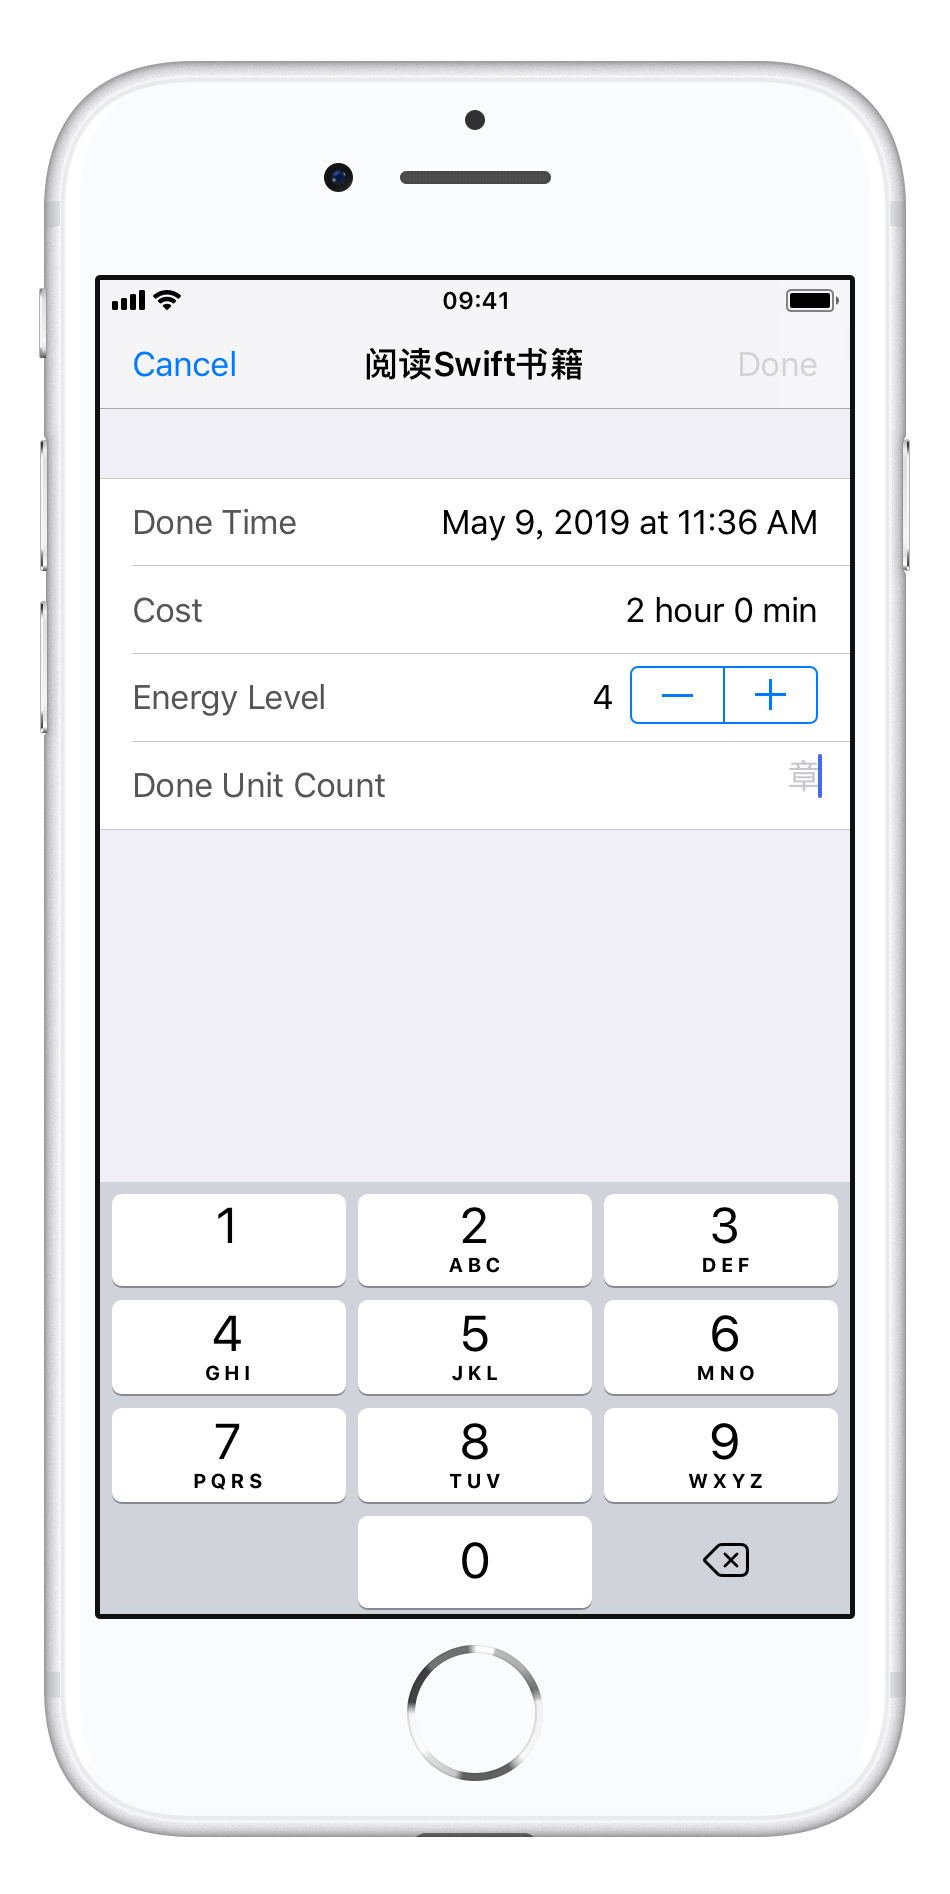
\includegraphics[height=10cm]{figure/system/add_action}}
	\caption{添加行为}
\end{figure}

\begin{lstlisting}[language={Swift}, caption={添加行为的代码}]
	let context = AppDelegate.viewContext
    let dateFormatter = DateFormatter()
    
    var action: Action? = nil
    var task: Task? = nil
    var doneTime = Date() {
        didSet {
            doneTimeLabel.text =
                dateFormatter.string(from: doneTime)
        }
    }
    var costMinutes = 0 {
        didSet {
            costLabel.text =
                String(format:"%d hour %d min", costMinutes/60, costMinutes%60)
        }
    }
    var energyLevel = 3 {
        didSet {
            energyLevelLabel.text = "\(energyLevel)"
            energyLevelStepper.value = Double(energyLevel)
        }
    }
    var doneUnitCount = 0 {
        didSet {
            doneUnitCountTextField.text =
                doneUnitCount == 0 ? "" : "\(doneUnitCount)"
            // TODO: calculate max from all actions
            if doneUnitCount > Int(task!.splitCount) {
                doneUnitCount = Int(task!.splitCount)
                doneUnitCountTextField.text = "\(doneUnitCount)"
            }
        }
    }
    @IBAction func cancelTapped(_ sender: UIBarButtonItem) {
        dismiss(animated: true, completion: nil)
    }
    @IBAction func doneTapped(_ sender: UIBarButtonItem) {
        if action == nil {
            action = Action(context: context)
        }
        action?.doneTime = doneTime
        action?.costMinutes = Int32(costMinutes)
        action?.energyLevel = Int16(energyLevel)
        action?.doneUnitCount = Int32(doneUnitCount)
        action?.task = task
        try? context.save()
        dismiss(animated: true, completion: nil)
    }
    @IBOutlet weak var doneButton: UIBarButtonItem!
    @IBOutlet weak var doneTimeLabel: PickerLabel!
    @IBOutlet weak var costLabel: PickerLabel!
    @IBOutlet weak var energyLevelLabel: UILabel!
    @IBOutlet weak var energyLevelStepper: UIStepper!
    @IBAction func energySetpperValueChanged(_ sender: UIStepper) {
        energyLevel = Int(energyLevelStepper.value)
    }
    @IBOutlet weak var doneUnitCountTextField: UITextField!
    @IBAction func doneUnitCountEditingChanged(_ sender: UITextField) {
        doneUnitCount = Int(doneUnitCountTextField.text!) ?? 0
        updateDoneButtonState()
    }
    
    override func viewDidLoad() {
        super.viewDidLoad()
        updateDoneButtonState()
        dateFormatter.dateStyle = .medium
        dateFormatter.timeStyle = .short
        self.title = task?.title
        if let action = action {
            task = action.task
            doneTime = action.doneTime ?? Date()
            costMinutes = Int(action.costMinutes)
            energyLevel = Int(action.energyLevel)
            doneUnitCount = Int(action.doneUnitCount)
        } else {
            doneTime = Date()
            costMinutes = Int(task!.costMinutes)
            energyLevel = Int(task!.energyLevel)
            doneUnitCountTextField.placeholder = task!.splitUnit
            doneUnitCountTextField.becomeFirstResponder()
        }
    }
    
    @objc func doneDateTimePickerValueChanged(sender: UIDatePicker) {
        doneTime = sender.date
    }
    
    @objc func costTimePickerValueChanged(sender: UIDatePicker) {
        costMinutes = Int(sender.countDownDuration/60)
    }
    
    func updateDoneButtonState() {
        let text = doneUnitCountTextField.text ?? ""
        doneButton.isEnabled = !text.isEmpty
    }
    
    // MARK: - Table view
    
    override func tableView(_ tableView: UITableView, didSelectRowAt indexPath: IndexPath) {
        tableView.deselectRow(at: indexPath, animated: true)
        switch indexPath.row {
        case 0:
            let datePicker = doneTimeLabel.inputView as? UIDatePicker
            datePicker?.datePickerMode = .dateAndTime
            datePicker?.addTarget(self, action: #selector(doneDateTimePickerValueChanged(sender:)), for: .valueChanged)
            doneTimeLabel.becomeFirstResponder()
            datePicker?.setDate(doneTime, animated: true)
        case 1:
            let datePicker = costLabel.inputView as? UIDatePicker
            datePicker?.datePickerMode = .countDownTimer
            datePicker?.minuteInterval = 5
            datePicker?.addTarget(self, action: #selector(costTimePickerValueChanged(sender:)), for: .valueChanged)
            costLabel.becomeFirstResponder()
            datePicker?.countDownDuration = TimeInterval(costMinutes*60)
        case 3:
            doneUnitCountTextField.becomeFirstResponder()
        default:
            break
        }
    }
\end{lstlisting}

这一界面与iOS 的健康添加行为的界面保持一致,将键盘作为DatePicker等输入的入口,
更符合用户的操作习惯。

为了更方便的管理行为,还提供了历史记录的查看。

\begin{figure}[H]
	\centering
	\makebox[\textwidth]{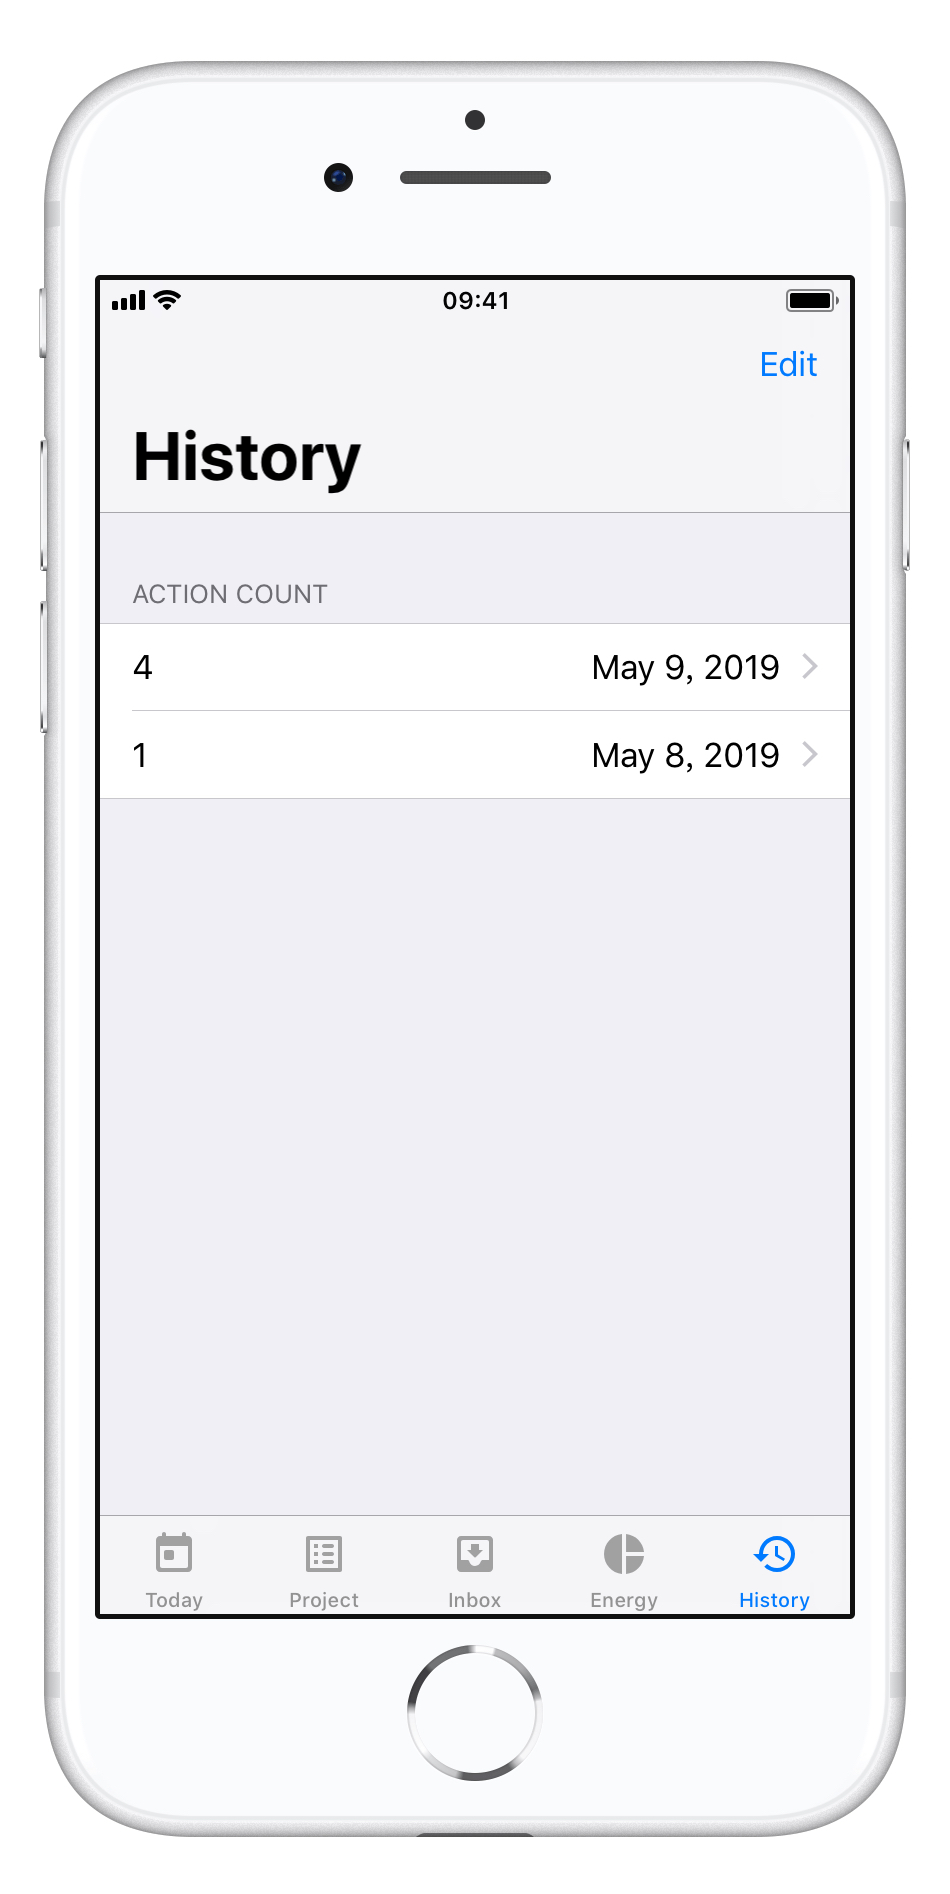
\includegraphics[height=10cm]{figure/system/history}}
	\caption{查看历史行为记录}
\end{figure}
%# -*- coding: utf-8-unix -*-
% !TEX program = xelatex
% !TEX root = ../thesis.tex
% !TEX encoding = UTF-8 Unicode

\chapter{系统测试}

对于任何软件,在完成了系统开发之后,都需要对系统进行测试,
以保证系统的质量。

\section{白盒测试}
本系统测试用例繁多,主要对以下几个较为重要的测试用例进行列举。
\begin{table}[H]
	\centering
	\caption{添加任务测试用例表}
	\begin{tabular}{p{3cm}p{3cm}p{3cm}p{3cm}} \toprule
	  操作步骤 & 预期结果 & 实际结果 & 比较 \\
	  \midrule
	  点击新建任务 & 弹出新建任务界面 & 弹出新建任务界面 & 通过 \\ \midrule
	  在新建任务界面点击任意日期选择行 & 在选择行下方弹出日期选择器 & 在选择行下方弹出日期选择器 & 通过 \\ \midrule
	  在新建任务界面点击增加或减少精力等级 & 精力等级跟随变动 & 精力等级跟随变动 & 通过 \\ \midrule
	  在新建任务界面点击增加拆分项目 & 在拆分数量行下放添加拆分数量单位输入框,同时将估计花费时间改为估计单位花费时间 & 在拆分数量行下放添加拆分数量单位输入框,同时将估计花费时间改为估计单位花费时间 & 通过 \\ \midrule
	  在新建任务界面点击选择项目 & 弹出选择项目界面 & 弹出选择项目界面 & 通过 \\ \midrule
	  在选择项目界面点击选择项目 & 跳转回新建任务界面,同时更新项目和任务依赖选择 & 跳转回新建任务界面,同时更新项目和任务依赖选择 & 通过 \\ \midrule
	  在新建任务界面点击选择依赖任务 & 弹出选任务选择界面 & 弹出选任务选择界面 & 通过 \\ \midrule
	  在任务选择界面选择依赖任务并返回 & 保存依赖任务到内存中并更新依赖任务提示栏 & 保存依赖任务到内存中并更新依赖任务提示栏 & 通过 \\ \midrule
	  在新建任务界面点击完成 & 保存任务跳并转回原界面 & 保存任务跳并转回原界面 & 通过 \\ \midrule
	  在新建任务界面点击取消 & 不保存任务跳并转回原界面 & 不保存任务跳并转回原界面 & 通过 \\ \midrule
	  \bottomrule
	\end{tabular}
\end{table}

\begin{table}[H]
	\centering
	\caption{用户完成含有拆分项目的任务用例表}
	\begin{tabular}{p{3cm}p{3cm}p{3cm}p{3cm}} \toprule
	  操作步骤 & 预期结果 & 实际结果 & 比较 \\
	  \midrule
	  点击完成任务 & 弹出新建行为界面 & 弹出新建行为界面 & 通过 \\ \midrule
	  在新建行为界面点击完成时间行 & 弹出日期和时间选择键盘 & 弹出日期和时间选择键盘 & 通过 \\ \midrule
	  在新建行为界面点击花费时间行 & 弹出倒计时时间选择键盘 & 弹出倒计时时间选择键盘 & 通过 \\ \midrule
	  在新建行为界面点击增加或减少精力等级 & 精力等级跟随变动 & 精力等级跟随变动 & 通过 \\ \midrule
	  在新建行为界面点击完成单位数量行 & 弹出数字键盘 & 弹出数字键盘 & 通过 \\ \midrule
	  在新建行为界面点击完成 & 保存行为跳并转回原界面 & 保存行为跳并转回原界面 & 通过 \\ \midrule
	  在新建行为界面点击取消 & 不保存行为跳并转回原界面 & 不保存行为跳并转回原界面 & 通过 \\ \midrule
	  \bottomrule
	\end{tabular}
\end{table}

\section{内存泄漏测试}
使用Xcode提供的Instruments对系统进行测试如下图所示
\begin{figure}[H]
	\centering
	\makebox[\textwidth]{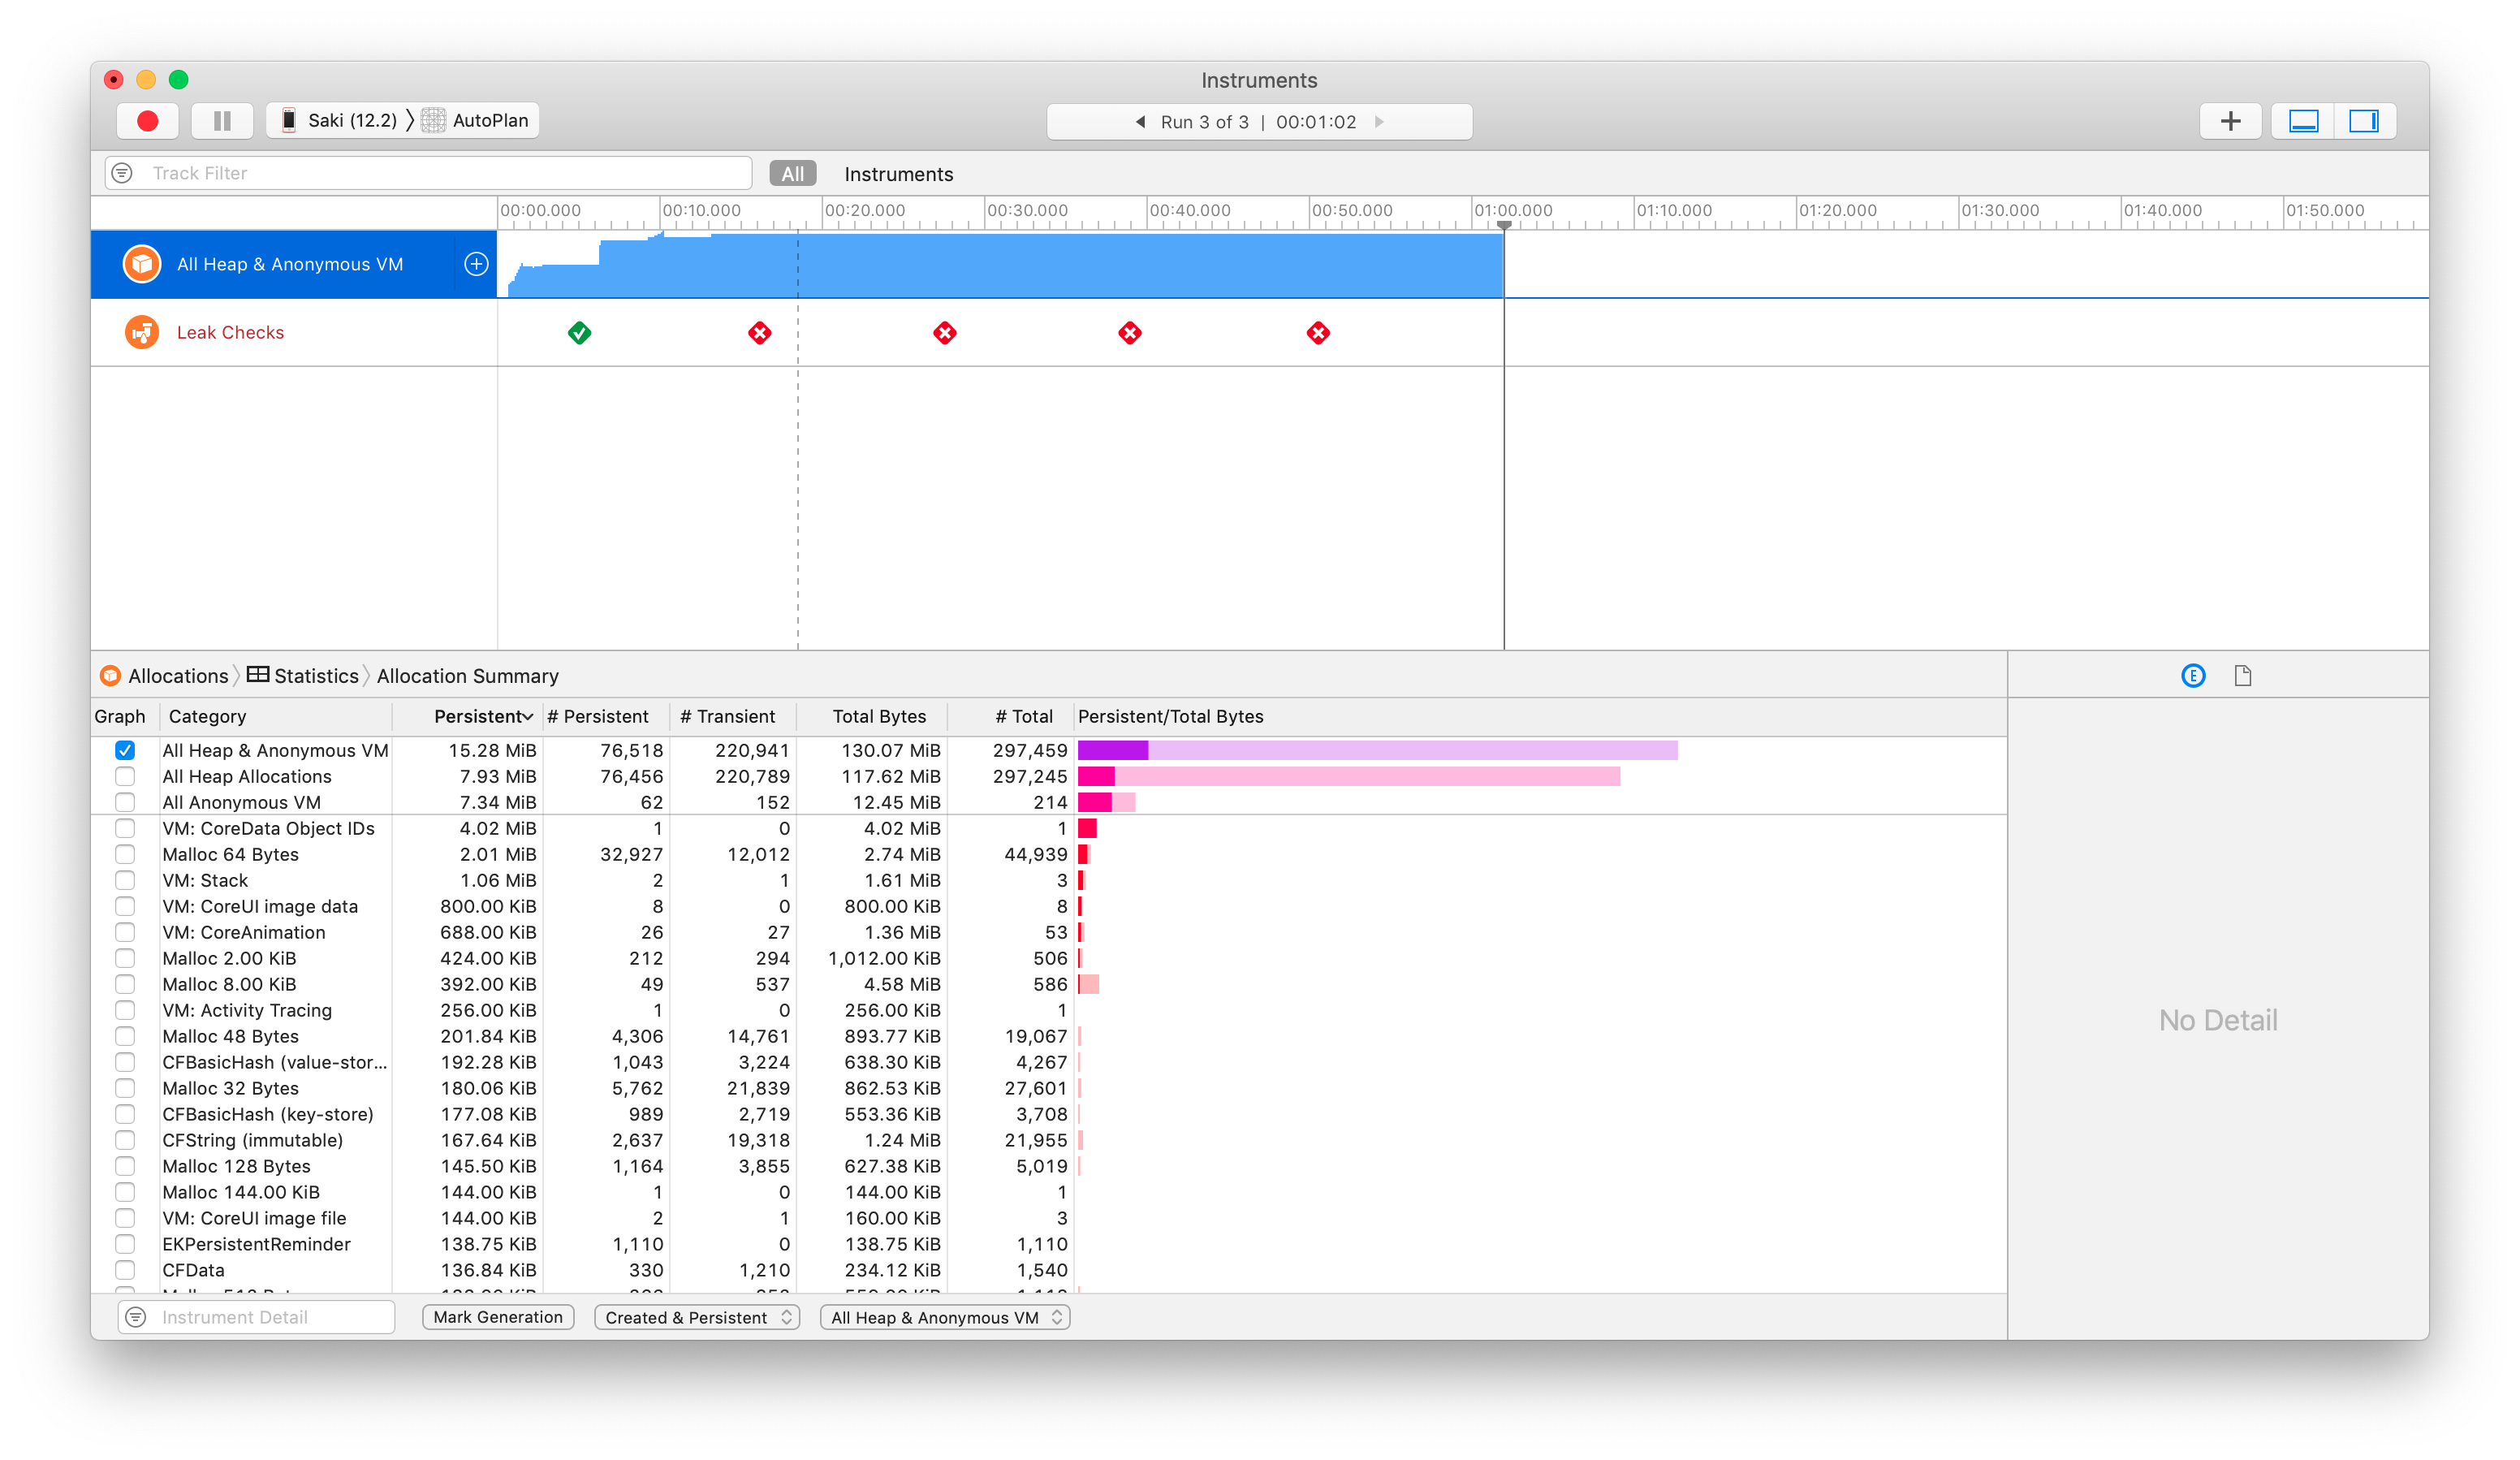
\includegraphics[width=\textwidth]{figure/test/memory_leak}}
	\caption{Instruments 内存泄漏测试}
\end{figure}
%# -*- coding: utf-8-unix -*-
% !TEX program = xelatex
% !TEX root = ../thesis.tex
% !TEX encoding = UTF-8 Unicode

\chapter{结论}

通过几个月的不断学习和摸索,初步掌握了iOS的开发,并完成了
本任务计划和时间管理系统的开发。此次毕业设计中我对自己有了新的认识,也明白了很多道理。
首先是对于系统总体的把握,虽然此次开发的是时间管理系统,但我个人对时间的把控却十分不足,
虽然也有一些客观因素,但主观上的眼高手低是造成问题的关键,而本系统也旨在通过对
任务的拆分和项目中任务的管理,帮助和我类似的人群解决这一问题。
我曾在Android平台上开发过类似的系统,但在开发本系统时却无法进行任何利用,这在跨平台开发上是也是需要值得深思的问题。
这也说明了对于一些看似相似的知识,没有经过自己实际运用和实践,就无法保证知识的有效性。

在开发过程中我也遇到了很多问题,但苦于iOS的普及程度远不如Android高,很多问题无法得到及时的解决,
在学习资料上的缺失和Swift语言的新颖导致我始终无法系统而有效的学习iOS开发。
比如在学习Auto Layout进行界面UI的搭建时,我很难指定出我想要的约束条件,通过翻阅Apple的开发者文档,才逐渐掌握。
但经过我的不懈努力,通过查找大量英文资料和视频,我独立解决了大部分问题,在和同学的探讨中我也学习到了一些有效的解决办法。
本次系统运用了面向对象的设计思想,采用标准的MVC架构,很大程度上提高了代码的可重用性和可维护性。
开发过程是漫长而枯燥的,但是看到最终的成品,还是令人激动,这对我来说是一次绝好的将理论知识运用于实践的过程。
不仅是软件开发的相关理论,还有个人的价值观和对任务管理及生活的思考,这个作品也是包含着我的思想的。

本系统完成了任务计划和时间管理的基本功能,但由于个人的水平有限,还有很多地方值得改进。
如界面设计可以更具个性,对于任务之间的依赖关系可以用图表表示地更加清晰,
为添加任务、添加项目、添加事件增加统一的新增入口,更加方便用户操作,
增强精力管理,使用户能清晰的看到精力分配的时间,加强下一步推荐的算法,为用户提供更为合理的任务提醒。
总之,通过本次毕业设计,我对于时间管理的开发有了更加深入的理解。

\backmatter % 文后无编号部分

\makeatletter

% 致谢
%# -*- coding: utf-8-unix -*-
% !TEX program = xelatex
% !TEX root = ../thesis.tex
% !TEX encoding = UTF-8 Unicode
%TC:ignore
\begin{thanks}

大学四年的学习生活即将结束,在本次毕业设计完成之际,
我要特别感谢我的指导老师李丽萍老师,老师秉承认真负责的工作态度,
在整个毕业设计过程中定时督促、检查我的系统完成情况,
从中指出我的不足之处,在我遇到困难时给予耐心的指导。
我能够完成系统的设计、编码和论文,还要感谢同学们的无私帮助。
非常感谢他们能够抽出时间,帮助我发现问题,解决问题,给出了很多有用的建议和补充。
最后,我由衷的感谢所有教导过我的老师们,
你们严谨的治学风格,让我很好的学习了专业知识;
你们独特的人格魅力,感染教导我为人处事。
还要感谢我的母校——上海第二工业大学四年来对我的精心培养,
让我能够变的更加出色,让我有自信成为社会的有用之才。

\end{thanks}
%TC:endignore
 

% 参考资料
\printbibliography[heading=bibintoc]

\makeatother

\end{document}
